\section{Improvement and robustification approaches}
\label{sec:res_improvement}
The results of Section \ref{sec:res_frames_motion} show the effects of scalloping loss can be attenuated by increasing the density of transmit beams. Although this method arguably is one of the most reliable way to reduce scalloping loss, it has several drawbacks. An increase in beams transmissions obviously results in longer image acquisition and processing time. This directly impacts the image frame rate (Table \ref{table:max_frame}). Additionally, Section \ref{sec:res_beams_motion} showed that this increased image acquisition time can result in loss of resolution with scatterer points moving in the medium.
Section \ref{sec:res_beams_motion} analyzed the effects of motion in the imaged medium during an image acquisition. Scatterer points motion can result in blur or distortion of their shape. The intensity of such distortions is dependent on the scatterer points velocity vector $\boldsymbol{v}_s$ relative to the one of the transmit beam distribution $\boldsymbol{v}_{tr}$.
The level of distortion, and therefore loss of resolution, intensifies as $\boldsymbol{v}_s$ converges towards $\boldsymbol{v}_{tr}$. This tendency is gives one more limitation to the increase of transmit beams.
Section \ref{sec:improvement} suggested several alternative approaches to reducing scalloping loss.

The first of these suggestions is to reduce the length of the transducers array. This length choice gives a trade-off between image resolution and scalloping loss magnitude. Figure \ref{fig:length_array} illustrates this statement by comparing two different array sizes for beam transmission. Besides the number of transducers used for beam transmission, all other parameters are common to both figures, including the size of the array for signal recording (96 elements).
In Figure \ref{fig:length_192}, scalloping loss is visible, but the two scatterer points are resolved. In Figure \ref{fig:length_24}, the smaller transmit array is not subject to visible, meaning higher than $1~dB$, scalloping loss. It is however unable to resolve the two scatterer points due to its relatively large mainlobe. Figure \ref{fig:length_array_all} shows that the array size is also pertinent for the other beamformers and yields a trade-off between resolution and scalloping loss as well, although to different extend for each beamformer.
Besides the trade-off between resolution and scalloping loss, this approach is not expected to yield any notable artifact and is therefore not further analyzed in this thesis.

\begin{figure}[ht]
    \centering
    \begin{subfigure}[t]{0.48\linewidth}
        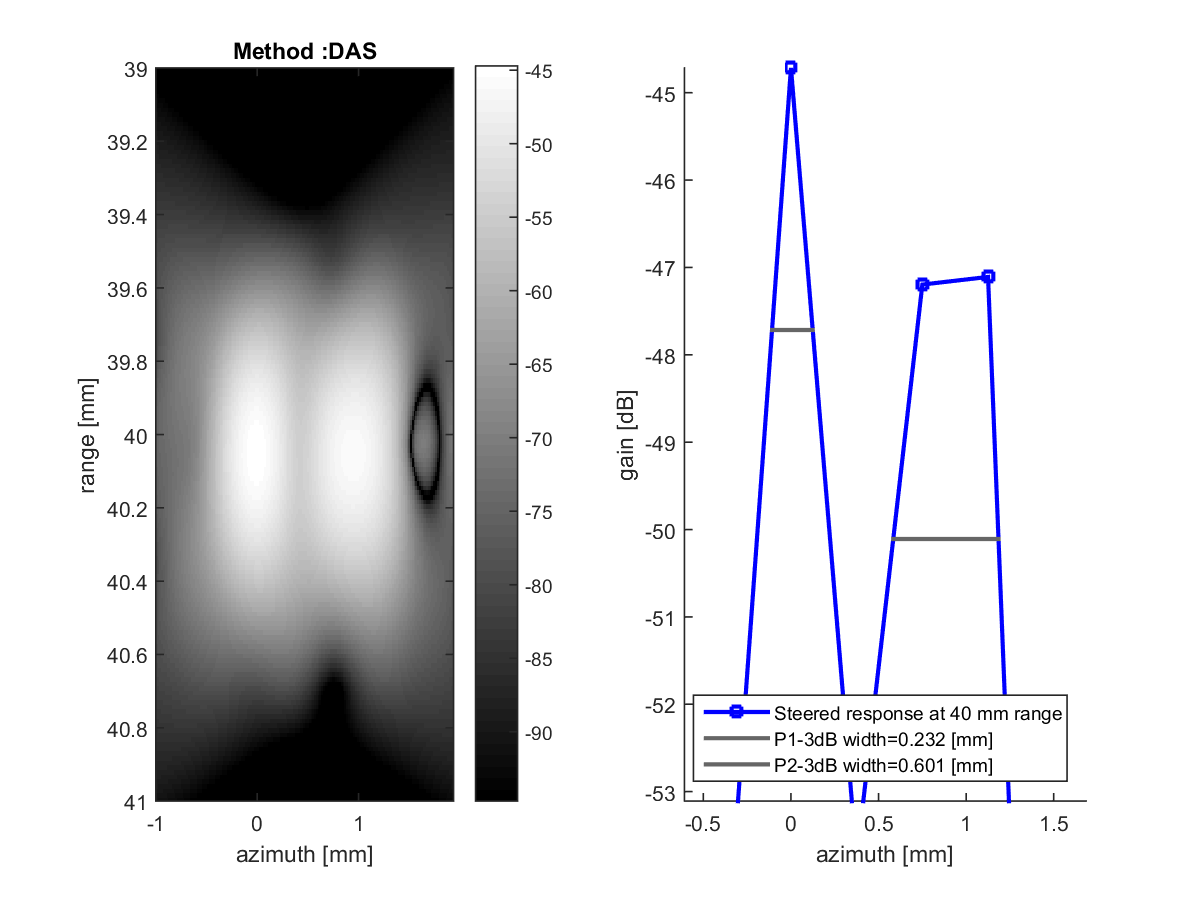
\includegraphics[width=\linewidth]{./images/discussion/DAS-doublesize.png}
        \caption{192 elements used for transmission}
        \label{fig:length_192}
    \end{subfigure}
    \quad
    \begin{subfigure}[t]{0.48\linewidth}
        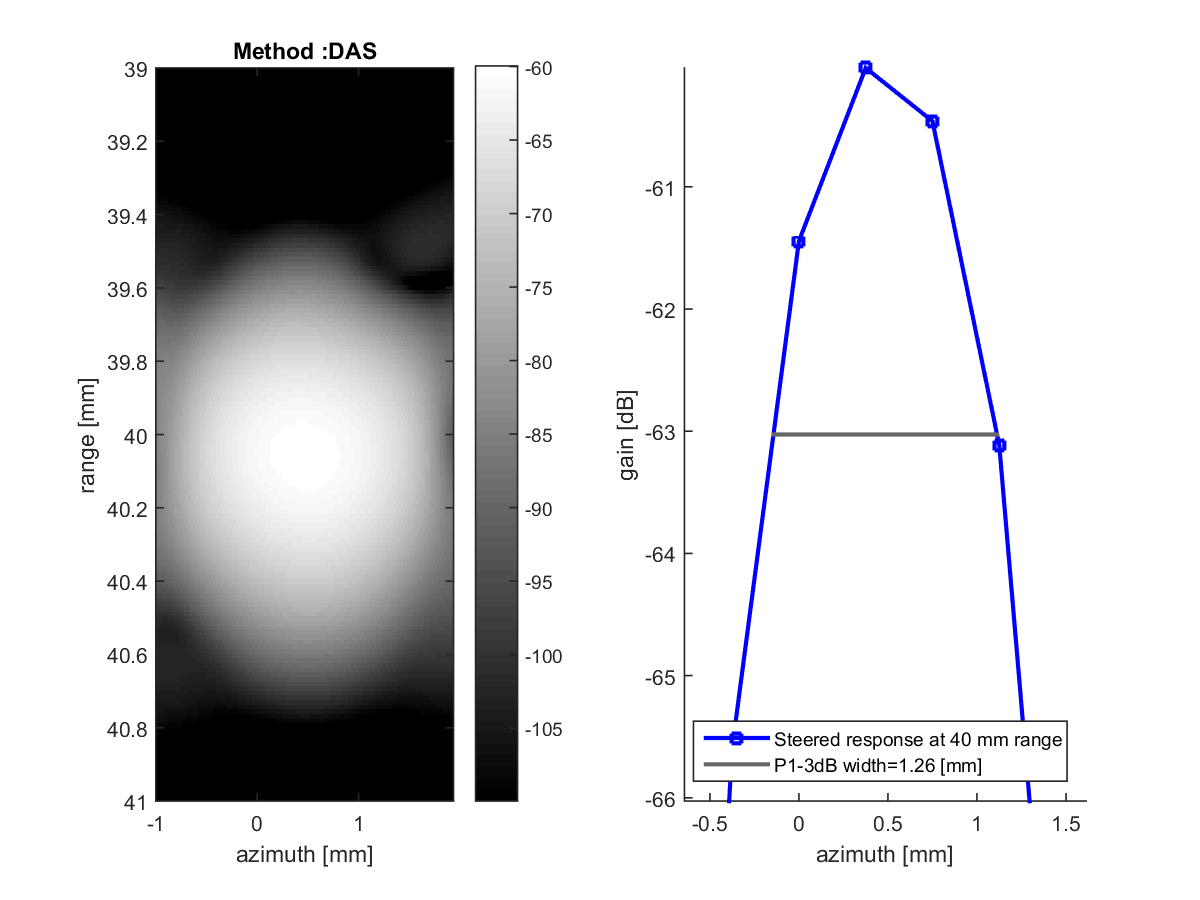
\includegraphics[width=\linewidth]{./images/discussion/DAS-fourthsize.png}
        \caption{24 elements used for transmission}
        \label{fig:length_24}
    \end{subfigure}
\caption{DAS beamformed image of two scatterer points $s_1$ and $s_2$ at focus range. $s_1$ on beam focus ($azimuth = 0~mm$), $s_2$ in between two beams ($azimuth = 0.9375~mm$)}
\label{fig:length_array}
\end{figure}

\begin{figure}[ht]
    \centering
    \begin{subfigure}[t]{0.48\linewidth}
        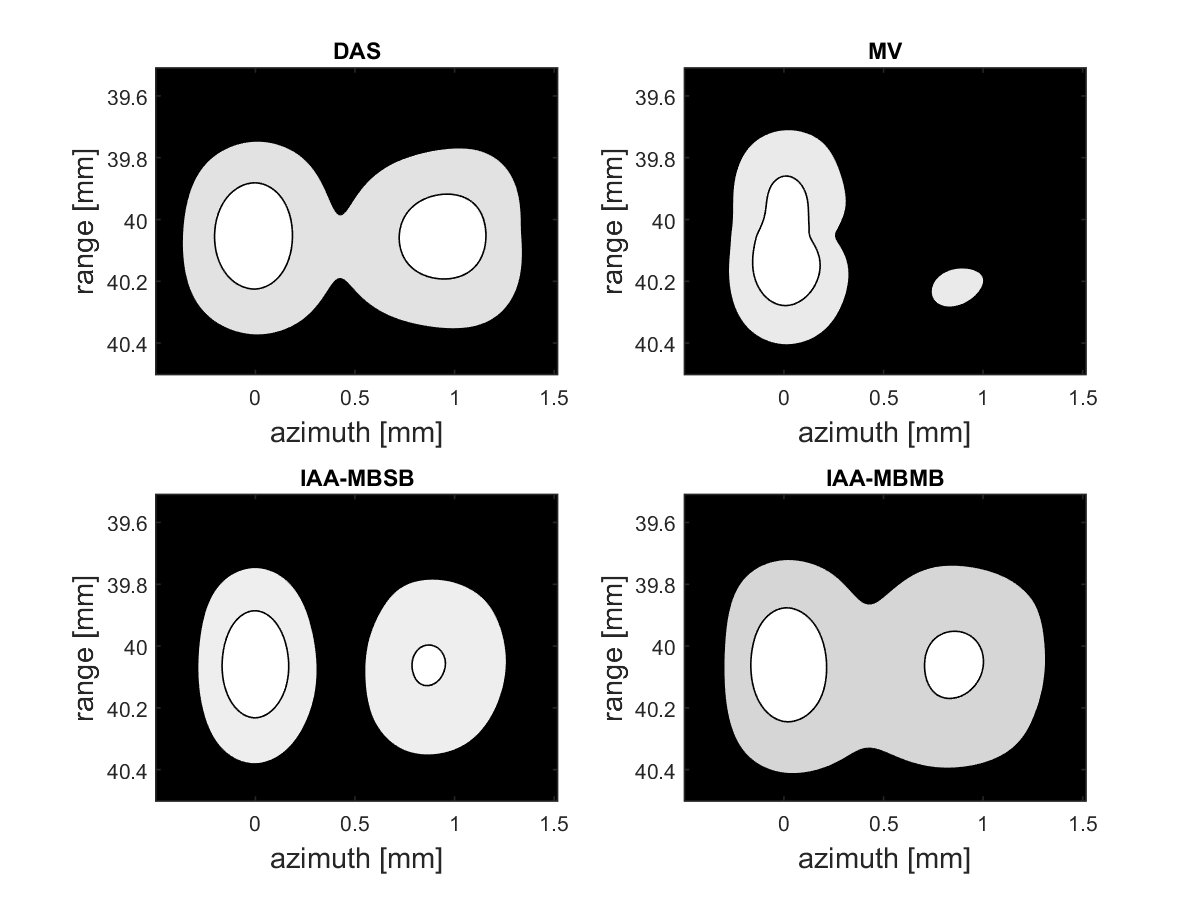
\includegraphics[width=\linewidth]{./images/discussion/all-doublesize.png}
        \caption{192 elements used for transmission}
    \end{subfigure}
    \quad
    \begin{subfigure}[t]{0.48\linewidth}
        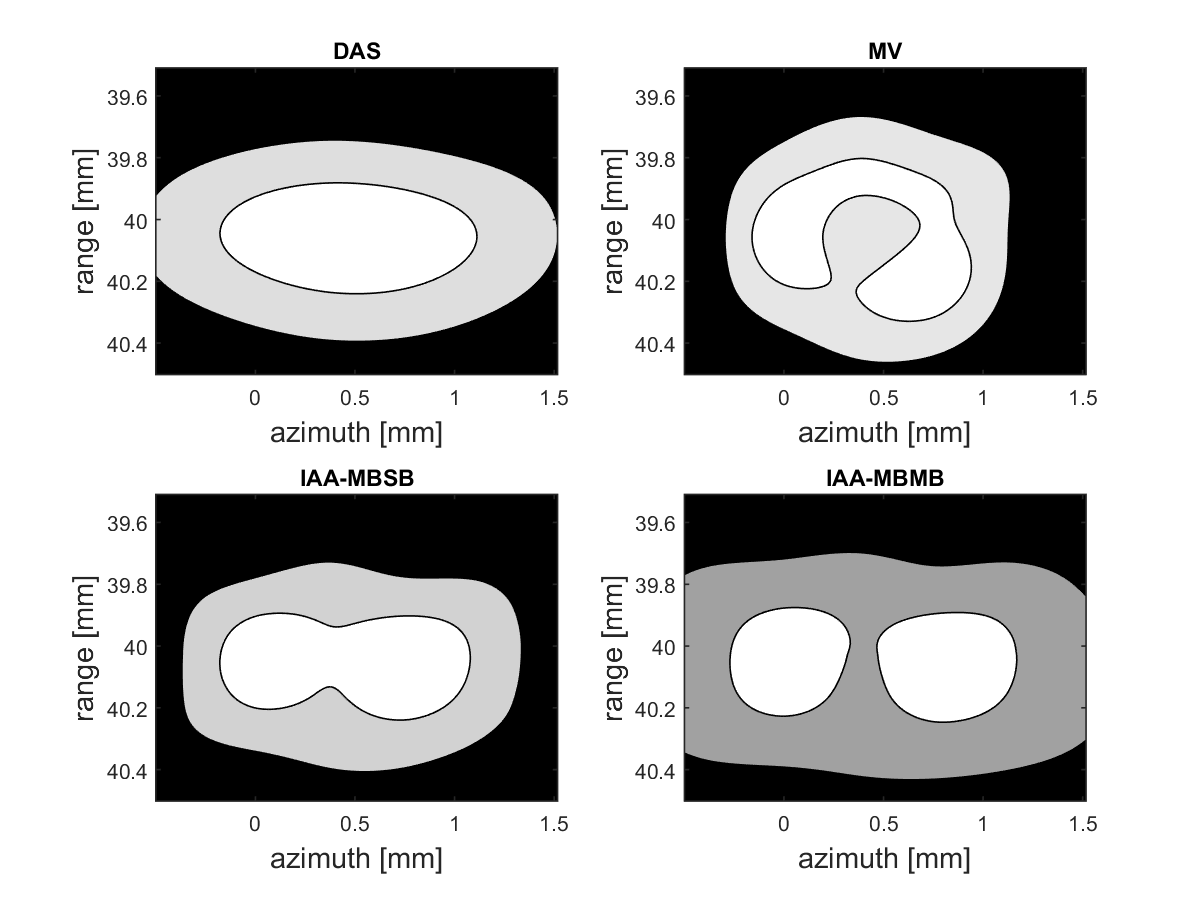
\includegraphics[width=\linewidth]{./images/discussion/all-fourthsize.png}
        \caption{24 elements used for transmission}
    \end{subfigure}
\caption{Contour plot of beamformed images of two scatterer points $s_1$ and $s_2$ at focus range. $s_1$ on beam focus ($azimuth = 0~mm$), $s_2$ in between two beams ($azimuth = 0.9375~mm$). Contour plot values: $max-100$, $max-10$ and $max-3~dB$}
\label{fig:length_array_all}
\end{figure}

Another alternative is to increase the density of receiving beams by signals time-delaying. This method is not able to recreate lost information, but it can combine the information of neighboring transmit beams.
Figure \ref{fig:time_upsampling_IAA} compares different variants of this approach with the IAA-MBMB beamformer. For each transmit beam, a set of $b_{re}$ receive beams is built such that $b_{re} = n \cdot b_{tr}, ~n = [1, 2, 5]$, which means that $n$ receive beams are built per transmit beam.

\begin{figure}[ht]
    \centering
    \begin{subfigure}[t]{0.48\linewidth}
        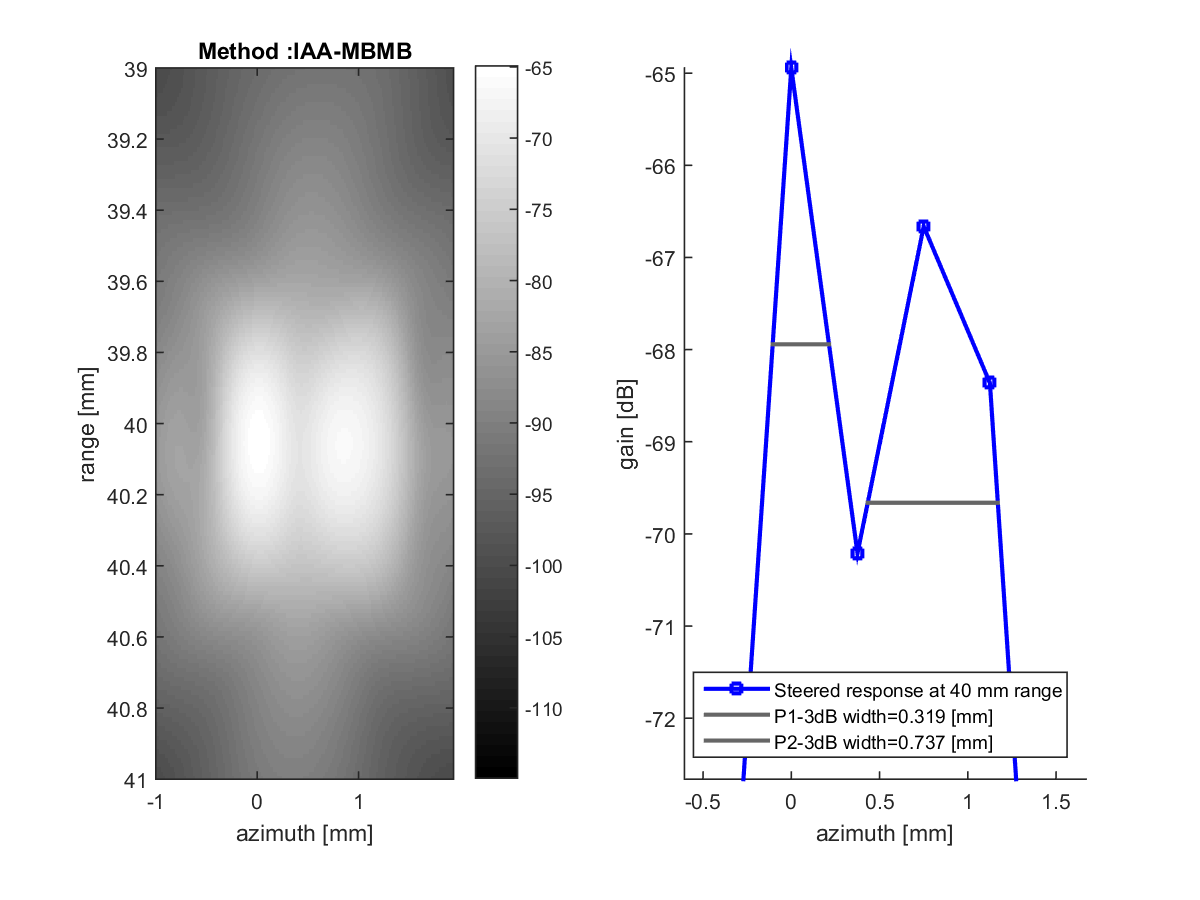
\includegraphics[width=\linewidth]{./images/discussion/IAA-MBMB-standard.png}
        \caption{No upsampling of receive beams. $b_{re} = b_{tr} = 65$}
    \end{subfigure}
        \label{fig:time1}
    \quad
    \begin{subfigure}[t]{0.48\linewidth}
        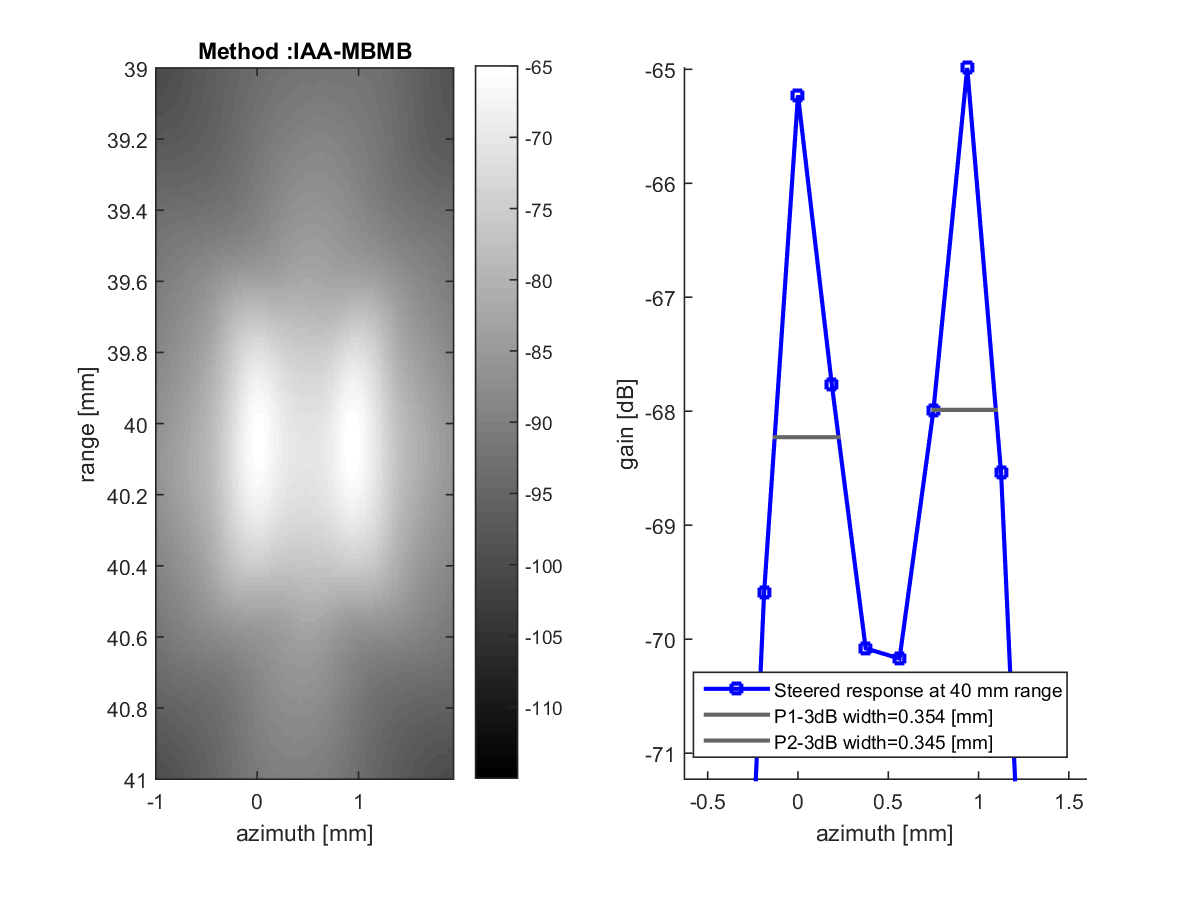
\includegraphics[width=\linewidth]{./images/discussion/IAA-MBMB-time2.png}
        \caption{Time-based upsampling by a factor of 2. $b_{re} = 2 \cdot 65 = 130$}
        \label{fig:time2}
    \end{subfigure}
    \quad
    \begin{subfigure}[t]{0.48\linewidth}
        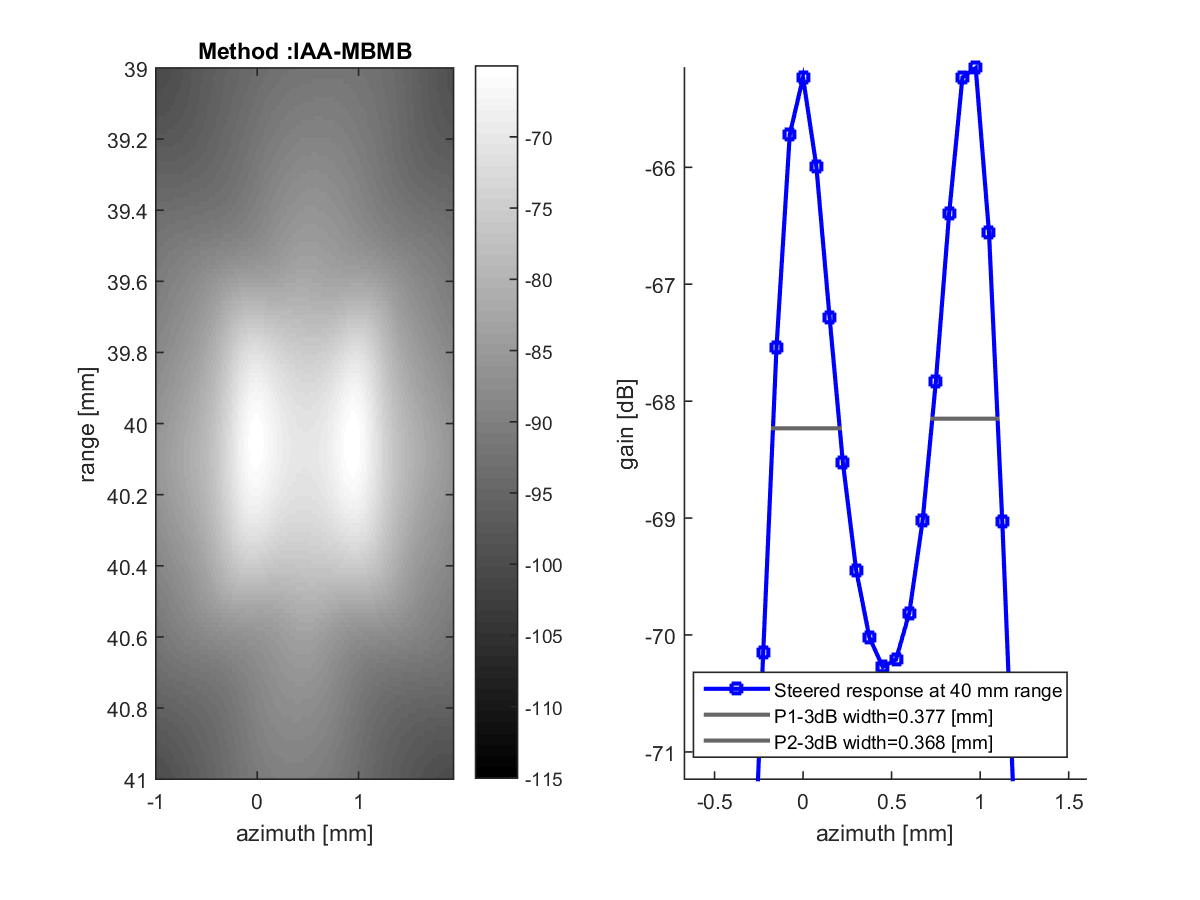
\includegraphics[width=\linewidth]{./images/discussion/IAA-MBMB-time4.png}
        \caption{Time-based upsampling by a factor of 4. $b_{re} = 4 \cdot 65 =  260$}
        \label{fig:time4}
    \end{subfigure}
\caption{IAA-MBMB beamformed images and steered responses of two scatterer points $s_1$ and $s_2$ at focus range. $s_1$ on beam focus ($azimuth = 0~mm$), $s_2$ in between two beams ($azimuth = 0.9375~mm$). Contour plot values: $max-100$, $max-10$ and $max-3~dB$}
\label{fig:time_upsampling_IAA}
\end{figure}

This approach obviously does not work if no energy is sent towards the receive beam focus direction. A great advantage of this approach is that it does not impact the image acquisition time, only its processing time. Considering its limitations and advantages, one could imaging a hybrid alternative. The transmit beams density could be set such that their mainlobe are guaranteed to intersect with their neighboring transmit beam mainlobe. This condition guarantees that energy is sent across the imaging sector. The receive beams density can then be increased to guarantee no visible scalloping loss. The implementation of such an approach falls outside of the scope of this thesis. One could for example start by assessing how big the transmit beams mainlobe intersection has to be for the time-delaying method to be able to reduce the effects of scalloping loss below the visibility threshold. Then similar experiments to those done in this thesis could be used to detect any potential artifact introduced by this approach.

Finally, the beamformers using the multibeam approach (Section \ref{sec:multibeam}) actively use phase-based shifting for receive beams focusing. The upsampling of receive beams presented here with time shifts can also be done to some extend with phase-based shifting (Section \ref{sec:beamforming_frequency}). \textbf{What is the difference with time-based shifting in this context? (Besides that they are done at different stages and maybe phase-based can achieve better computational efficiency(?))}
This approach is probably subject to the same limitations than the time-based focusing approach in addition to being limited to small phase shifts. Figure \ref{fig:phase_upsampling} gives an example of the use of phase-based upsampling to correct for scalloping loss. The scenario is similar to the one of Figure \ref{fig:time_upsampling}, with an array of 96 elements used for both transmission and reception.

Figures \ref{fig:phase2} and \ref{fig:phase4} reveal an noticeable improvement in both image resolution and scalloping loss correction compared to that of Figure \ref{fig:phase1}. The performances of phase-based upsampling are extremely similar to those of time-based upsampling (Figure \ref{fig:time_upsampling}). They also show that the receive beam density does not necessarily have to be very high to achieve high resolvability.
A similar hybrid solution as suggested for time-based upsampling could be experimented with phase-based upsampling.
Figure \ref{fig:linear_motion_double_upsampled} repeats the experiments of Figure \ref{fig:linear_motion_double} with the use of phase-based upsampling. The enhanced scalloping loss correction allows for better resolvability capacities and increased robustness to motion in the imaged medium. The approach of increasing the receive beams density does not have any impact on the image acquisition time, which is why it does not result in any additional artifact with the presence of motion. The main negative consequence of increasing the receive beams density is an increased computation load, which can relatively easily be overcome with appropriate hardware and efficient algorithm implementation.

\begin{figure}[ht]
    \centering
    \begin{subfigure}[t]{0.48\linewidth}
        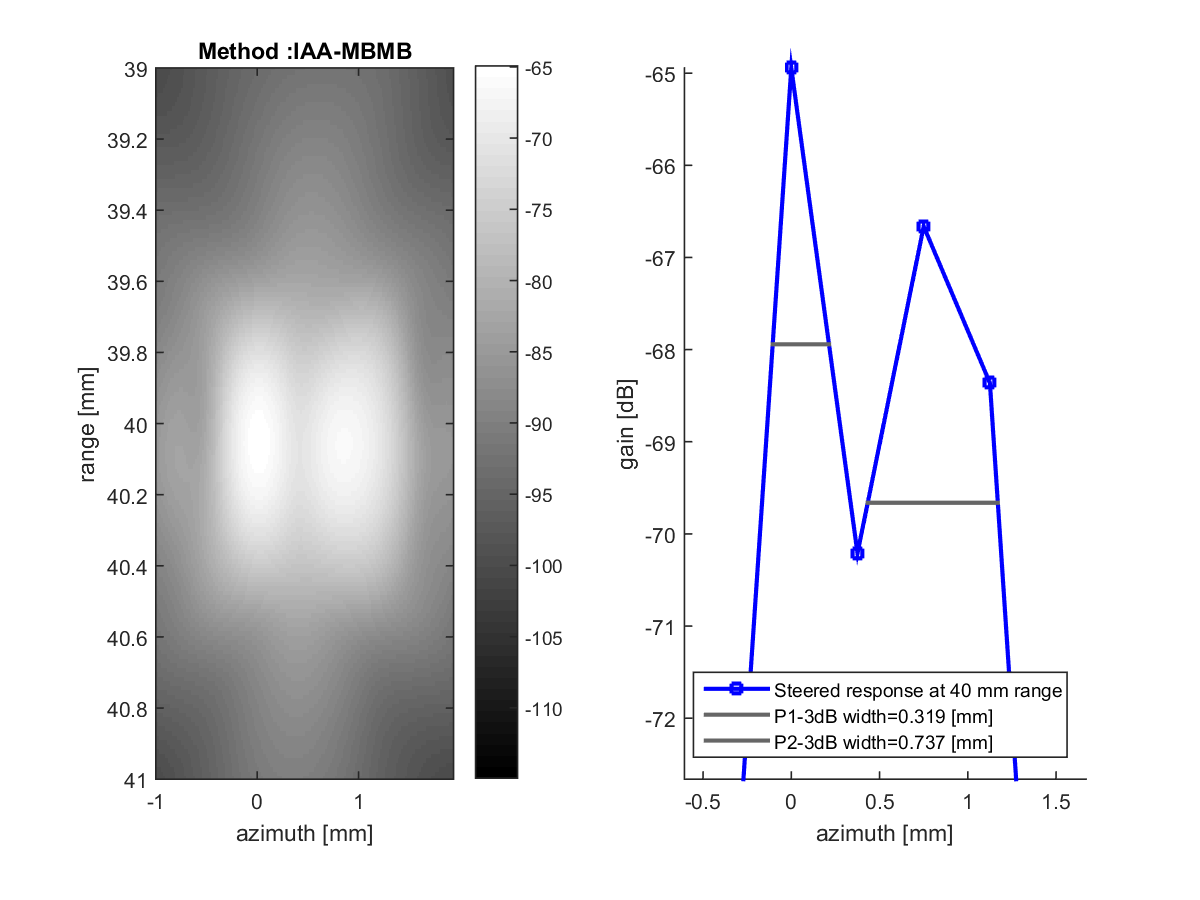
\includegraphics[width=\linewidth]{./images/discussion/IAA-MBMB-standard.png}
        \caption{No upsampling of receive beams. $b_{re} = b_{tr} = 65$}
        \label{fig:phase1}
    \end{subfigure}
    \quad
    \begin{subfigure}[t]{0.48\linewidth}
        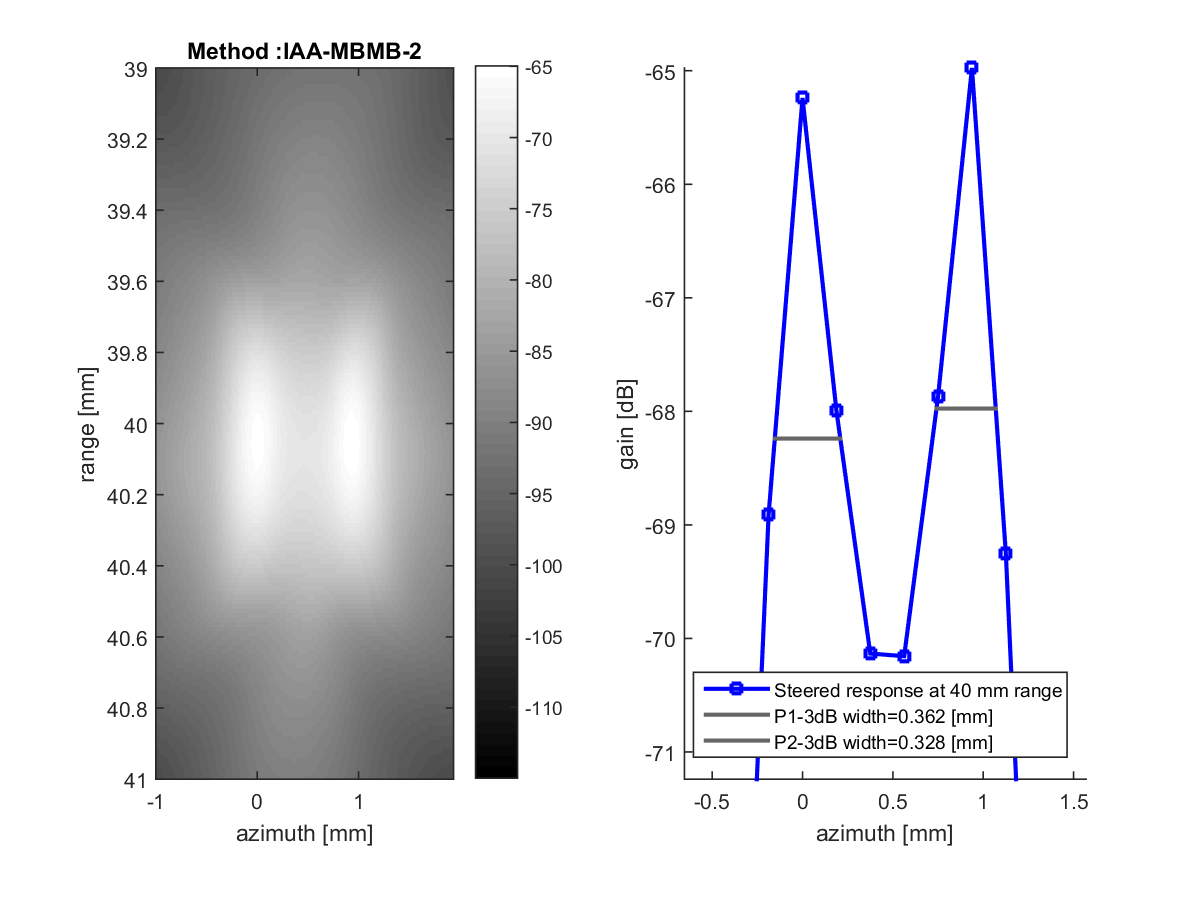
\includegraphics[width=\linewidth]{./images/discussion/IAA-MBMB-phase2.png}
        \caption{Phase-based upsampling by a factor of 2. $b_{re} = 2 \cdot 65 = 130$}
        \label{fig:phase2}
    \end{subfigure}
    \quad
    \begin{subfigure}[t]{0.48\linewidth}
        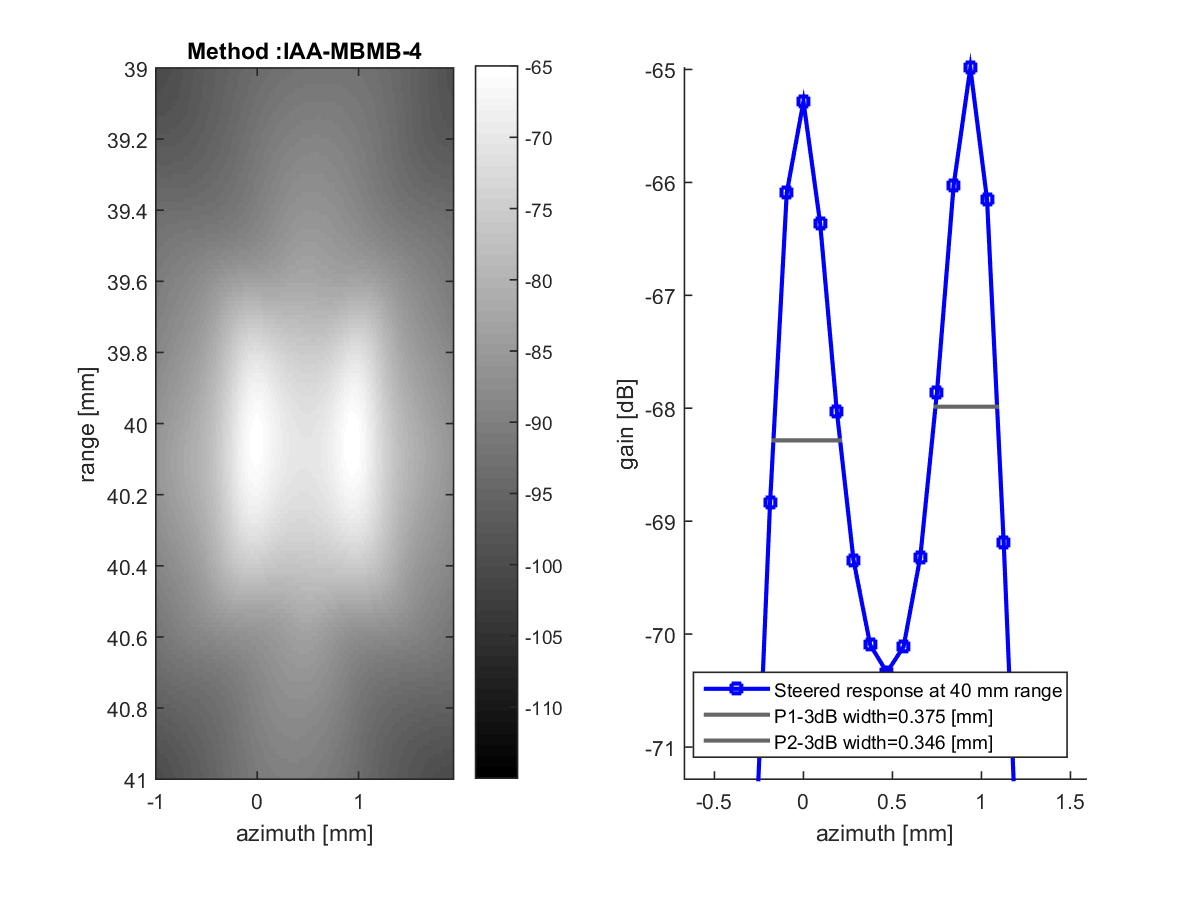
\includegraphics[width=\linewidth]{./images/discussion/IAA-MBMB-phase4.png}
        \caption{Phase-based upsampling by a factor of 4. $b_{re} = 4 \cdot 65 =  260$}
        \label{fig:phase4}
    \end{subfigure}
\caption{IAA-MBMB beamformed images and steered responses of two scatterer points $s_1$ and $s_2$ at focus range. $s_1$ on beam focus ($azimuth = 0~mm$), $s_2$ in between two beams ($azimuth = 0.9375~mm$). Contour plot values: $max-100$, $max-10$ and $max-3~dB$}
\label{fig:phase_upsampling}
\end{figure}


\begin{figure}[ht]
    \centering
    \begin{subfigure}[t]{0.48\linewidth}
        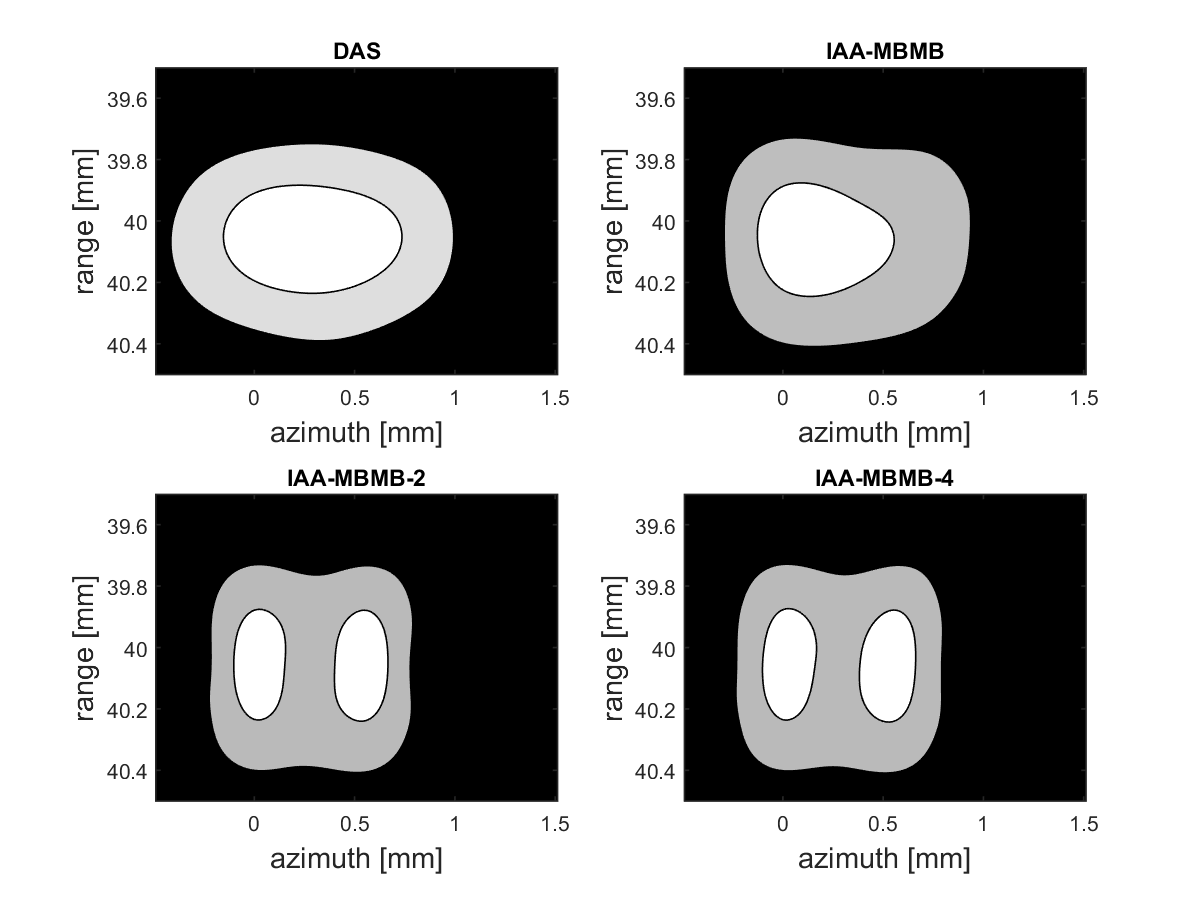
\includegraphics[width=\linewidth]{./images/results/3/motion_0_-06.png}
        \caption{$\boldsymbol{v}_s = (-0.6, 0)~m/s$}
        \label{fig:double_lateral}
    \end{subfigure}
    \quad
    \begin{subfigure}[t]{0.48\linewidth}
        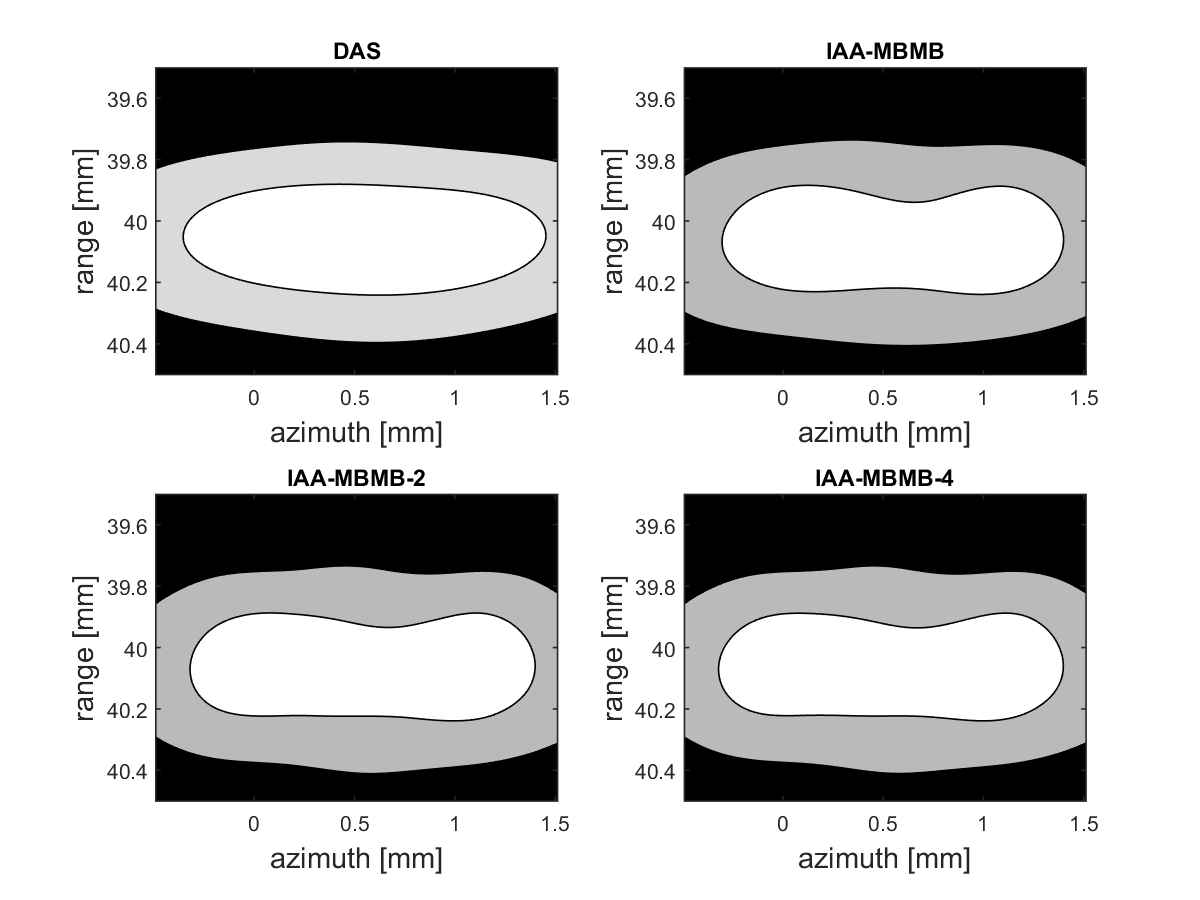
\includegraphics[width=\linewidth]{./images/results/3/motion_0_06.png}
        \caption{$\boldsymbol{v}_s = (0.6, 0)~m/s$}
    \end{subfigure}
    \quad
    \begin{subfigure}[t]{0.48\linewidth}
        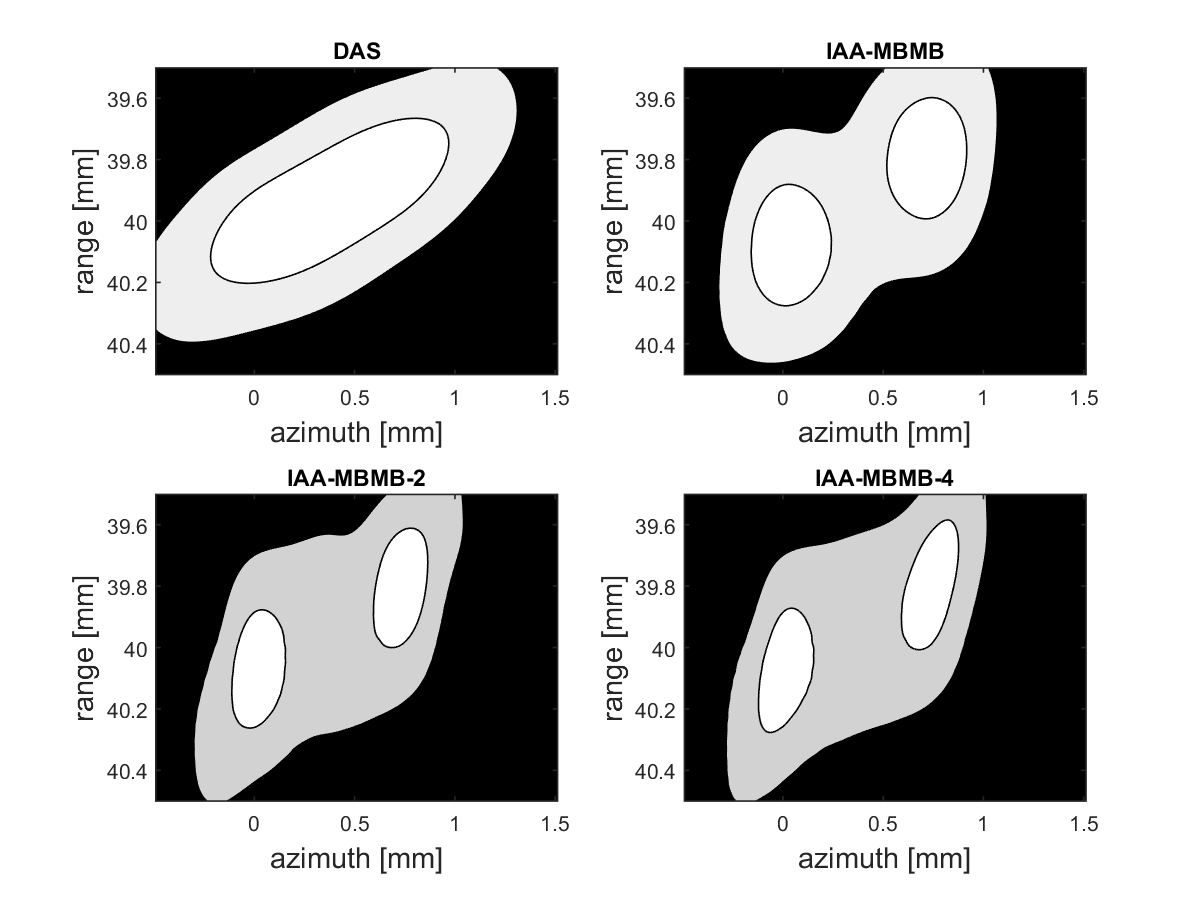
\includegraphics[width=\linewidth]{./images/results/3/motion_90_-06.png}
        \caption{$\boldsymbol{v}_s = (0, -0.6)~m/s$}
    \end{subfigure}
    \quad
    \begin{subfigure}[t]{0.48\linewidth}
        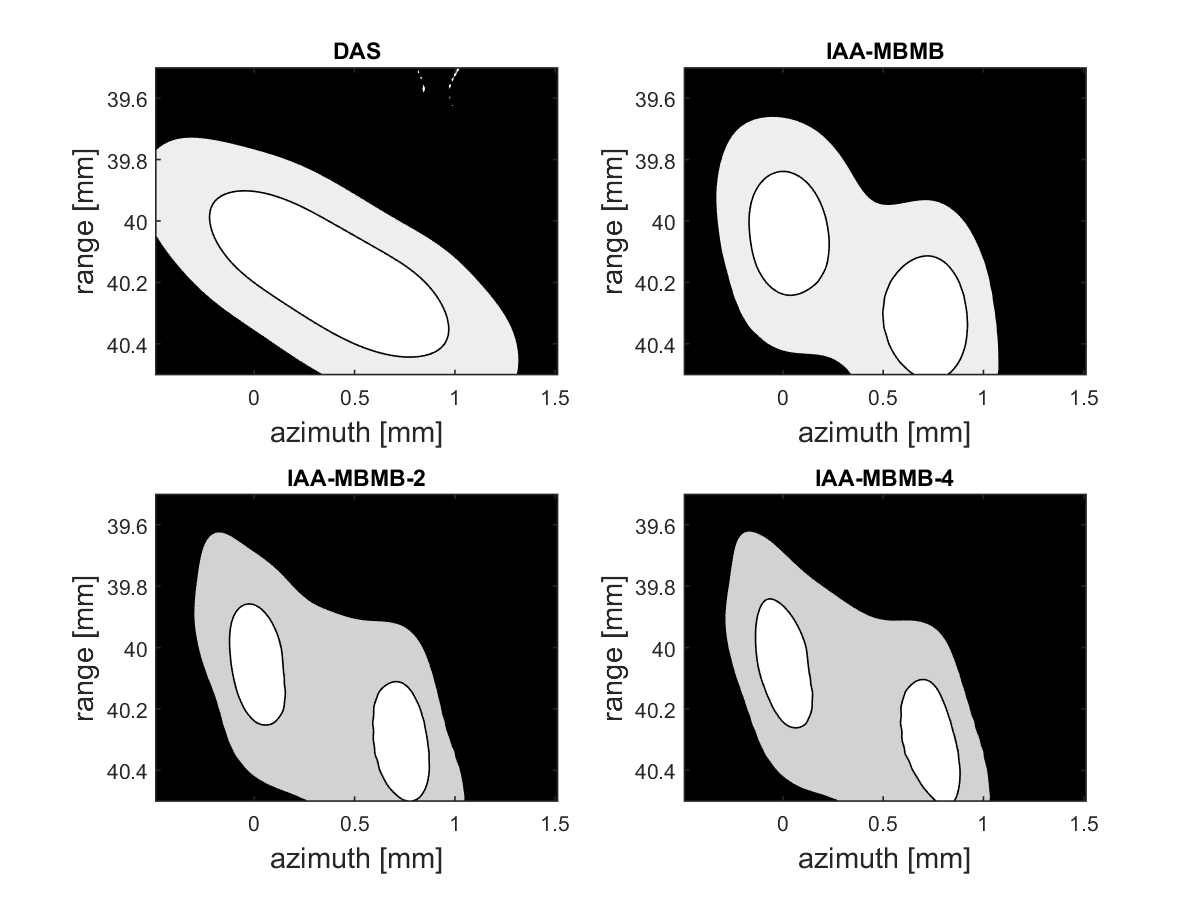
\includegraphics[width=\linewidth]{./images/results/3/motion_90_06.png}
        \caption{$\boldsymbol{v}_s = (0, 0.6)~m/s$}
    \end{subfigure}
    \quad
    \begin{subfigure}[t]{0.48\linewidth}
        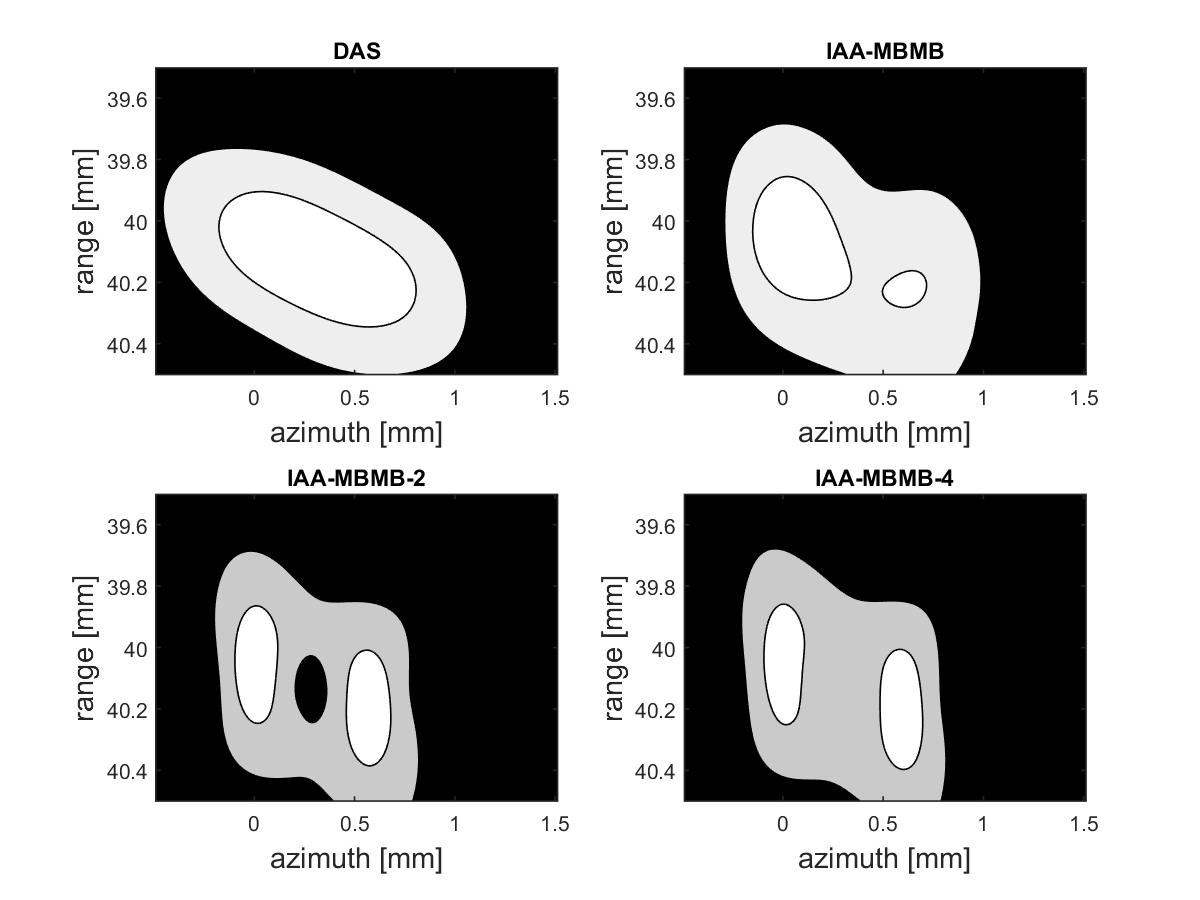
\includegraphics[width=\linewidth]{./images/results/3/motion_-45_-06.png}
        \caption{$\boldsymbol{v}_s = (-0.42, 0.42)~m/s$}
        \label{fig:double_diag1}
    \end{subfigure}
    \quad
    \begin{subfigure}[t]{0.48\linewidth}
        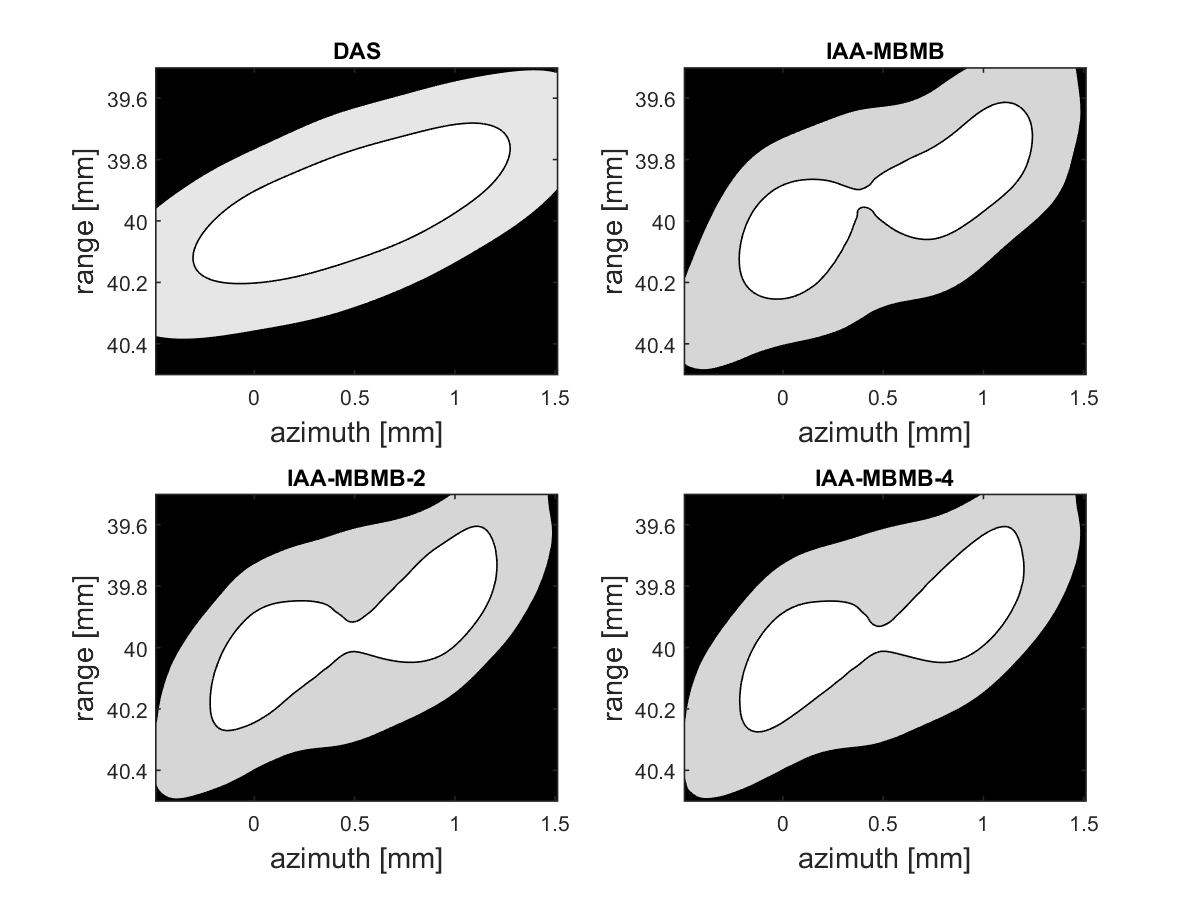
\includegraphics[width=\linewidth]{./images/results/3/motion_-45_06.png}
        \caption{$\boldsymbol{v}_s = (0.42, -0.42)~m/s$}
    \end{subfigure}
    \quad
    \begin{subfigure}[t]{0.48\linewidth}
        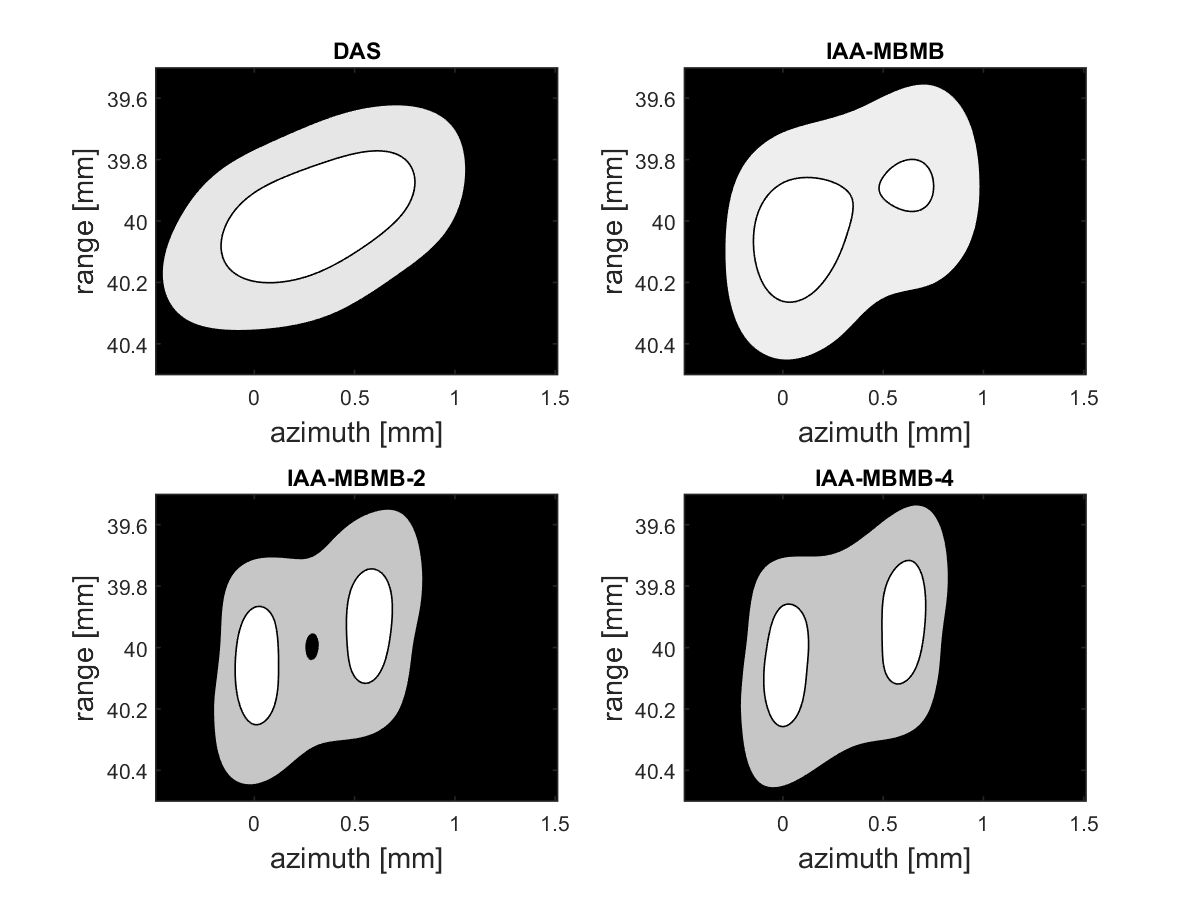
\includegraphics[width=\linewidth]{./images/results/3/motion_45_-06.png}
        \caption{$\boldsymbol{v}_s = (-0.42, -0.42)~m/s$}
        \label{fig:double_diag2}
    \end{subfigure}
    \quad
    \begin{subfigure}[t]{0.48\linewidth}
        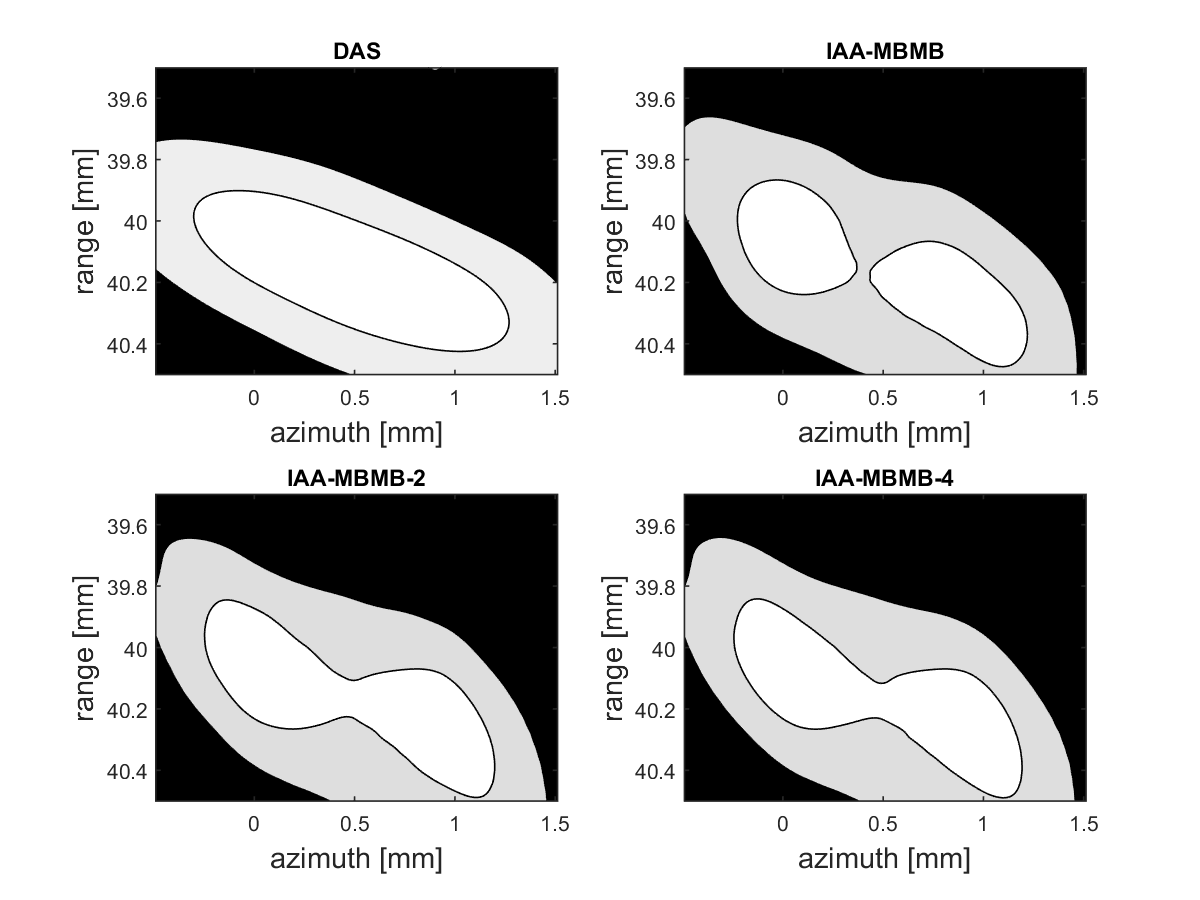
\includegraphics[width=\linewidth]{./images/results/3/motion_45_06.png}
        \caption{$\boldsymbol{v}_s = (0.42, 0.42)~m/s$}
    \end{subfigure}
	\caption{Two scatterer points in various linear motions $\boldsymbol{v}_s$ with $|\boldsymbol{v}_s|=0.6~m/s$ in noiseless medium. The algorithms compared are DAS, IAA-MBMB, IAA-MBMB with $b_{re} = 2 \cdot b_{tr} = 130$ and IAA-MBMB with $b_{re} = 5 \cdot b_{tr} = 325$. Contour plot levels: max-100, max-10 and max-3 dB}
	\label{fig:linear_motion_double_upsampled}
\end{figure}









\iffalse

\begin{figure}[ht]
    \centering
    \begin{subfigure}[t]{0.48\linewidth}
        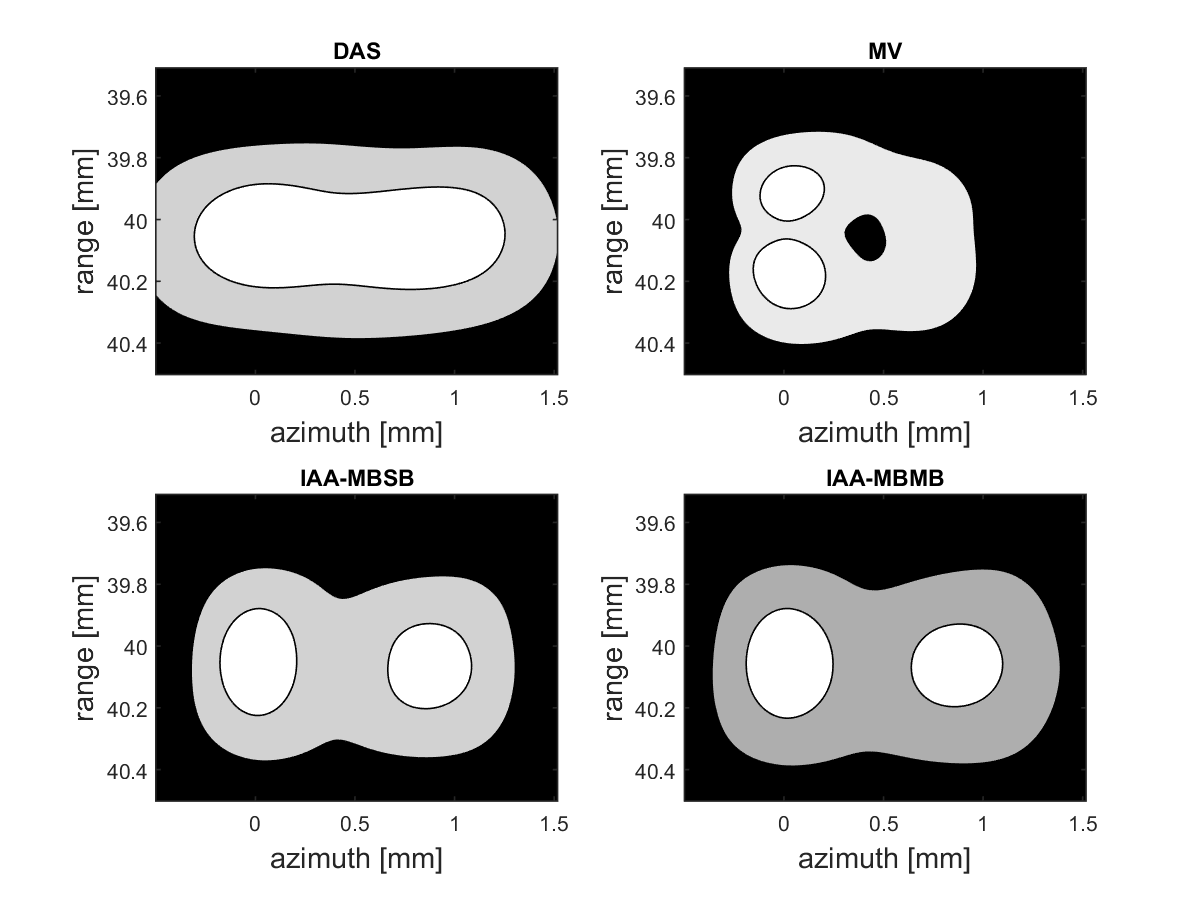
\includegraphics[width=\linewidth]{./images/discussion/all-standard.png}
        \caption{96 elements used for transmission. No upsampling of receive beams. $b_{re} = b_{tr} = 65$}
    \end{subfigure}
    \quad
    \begin{subfigure}[t]{0.48\linewidth}
        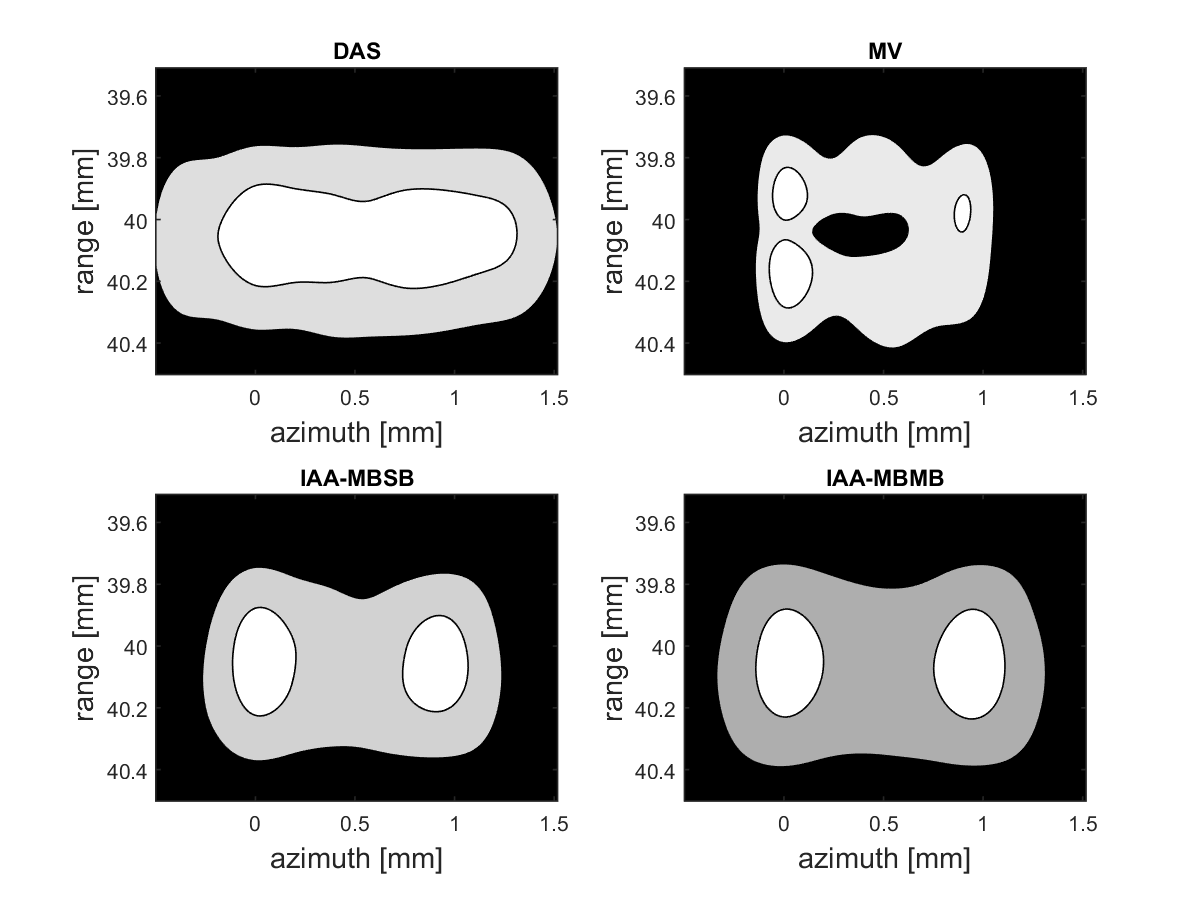
\includegraphics[width=\linewidth]{./images/discussion/all-time2.png}
        \caption{Upsampling by a factor of 2. $b_{re} = 2 \cdot 65 = 130$}
    \end{subfigure}
    \quad
    \begin{subfigure}[t]{0.48\linewidth}
        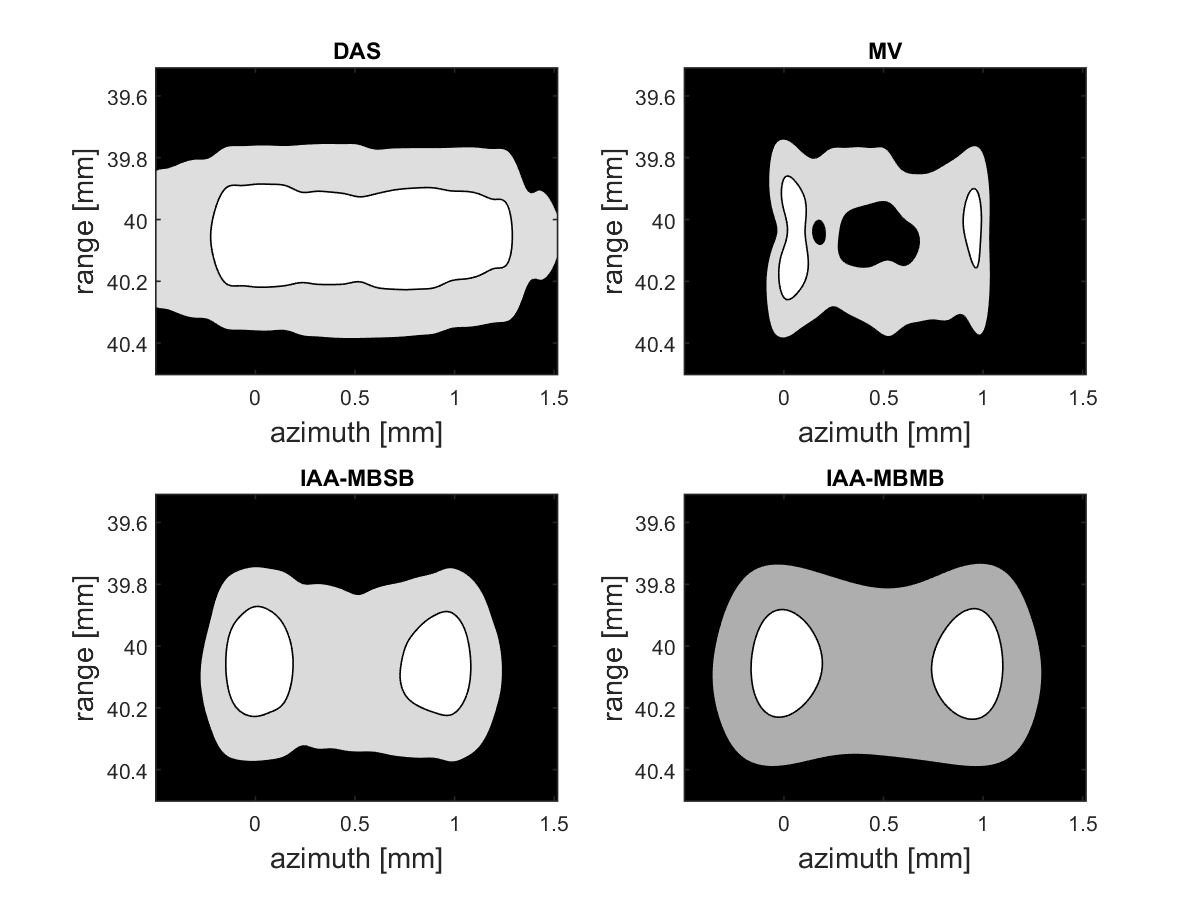
\includegraphics[width=\linewidth]{./images/discussion/all-time5.png}
        \caption{Upsampling by a factor of 5. $b_{re} = 5 \cdot 65 =  325$}
    \end{subfigure}
\caption{Contour plot of beamformed images of two scatterer points $s_1$ and $s_2$ at focus range. $s_1$ on beam focus ($azimuth = 0~mm$), $s_2$ in between two beams ($azimuth = 0.9375~mm$). Contour plot values: $max-100$, $max-10$ and $max-3~dB$}
\label{fig:time_upsampling}
\end{figure}




\begin{figure}[ht]
    \centering
    \begin{subfigure}[t]{0.48\linewidth}
        \includegraphics[width=\linewidth]{./images/discussion/all-phase2.png}
        \caption{Phase-based upsampling by a factor of 2. $b_{re} = 2 \cdot 65 = 130$}
    \end{subfigure}
    \quad
    \begin{subfigure}[t]{0.48\linewidth}
        \includegraphics[width=\linewidth]{./images/discussion/all-phase5.png}
        \caption{Phase-based upsampling by a factor of 5. $b_{re} = 5 \cdot 65 =  325$}
    \end{subfigure}
\caption{Contour plot of beamformed images of two scatterer points $s_1$ and $s_2$ at focus range. $s_1$ on beam focus ($azimuth = 0~mm$), $s_2$ in between two beams ($azimuth = 0.9375~mm$). Contour plot values: $max-100$, $max-10$ and $max-3~dB$}
\label{fig:phase_upsampling}
\end{figure}
Those results are extremely positive and are worth a deeper analysis of the approach. The analysis of Sections \ref{sec:res_frames_motion} and \ref{sec:res_beams_motion} are reproduced with the use of phase-based shifting for upsampling of receive beams. The analysis is focused on the IAA-MBMB beamformer with different upsampling values. This section compares the following algorithms:
\begin{itemize}
    \item DAS: The DAS results from previous sections are reproduced here as a comparison reference
    \item IAA-MBMB: The IAA-MBMB is also kept as in previous sections. The receive beams density and orientation matches the ones of the transmit beams
    \item IAA-MBMB-2: The number of receive beams is doubled compared to the number of transmit beams
    \item IAA-MBMB-4: The number of receive beams is four times the number of transmit beams
\end{itemize}
\noindent
The initial assumptions made in Section \ref{sec:res_frames_motion} need to be tested once again. Figures \ref{fig:loss_vs_shift_upsampled} and \ref{fig:loss_vs_range_upsampled} are produced in the same manner as Figures \ref{fig:loss_vs_shift} and \ref{fig:loss_vs_range}. Figure \ref{fig:loss_vs_shift_upsampled} reveals that, unlike for previous experiments, the maximum scalloping loss is not always happening exactly in between two transmit beams. For that reason several scatterer point positions are simulated are compared to estimate the maximum scalloping loss. Each frame is simulated with the scatterer point along the beamformer focus range at different angles $\theta_s$. If $\theta_b$ is the angular difference between two beams, the different frames are simulated with $\theta_s = 0$, $\theta_b / 4$, $\theta_b / 2$ or $3 \theta_b / 4$.
Figure \ref{fig:loss_vs_range_upsampled} shows that the maximum scalloping loss still occurs at focus range for most beamformers. The comparison of the IAA-MBMB, IAA-MBMB-2 and IAA-MBMB-4 results might suggest that as the upsampling factor $F_{up}$ goes to infinity, the curves converge towards a zero-valued line. This supposition is not verified in the scope of this thesis.

\begin{figure}[ht]
    \centering
    \begin{subfigure}[t]{0.48\linewidth}
        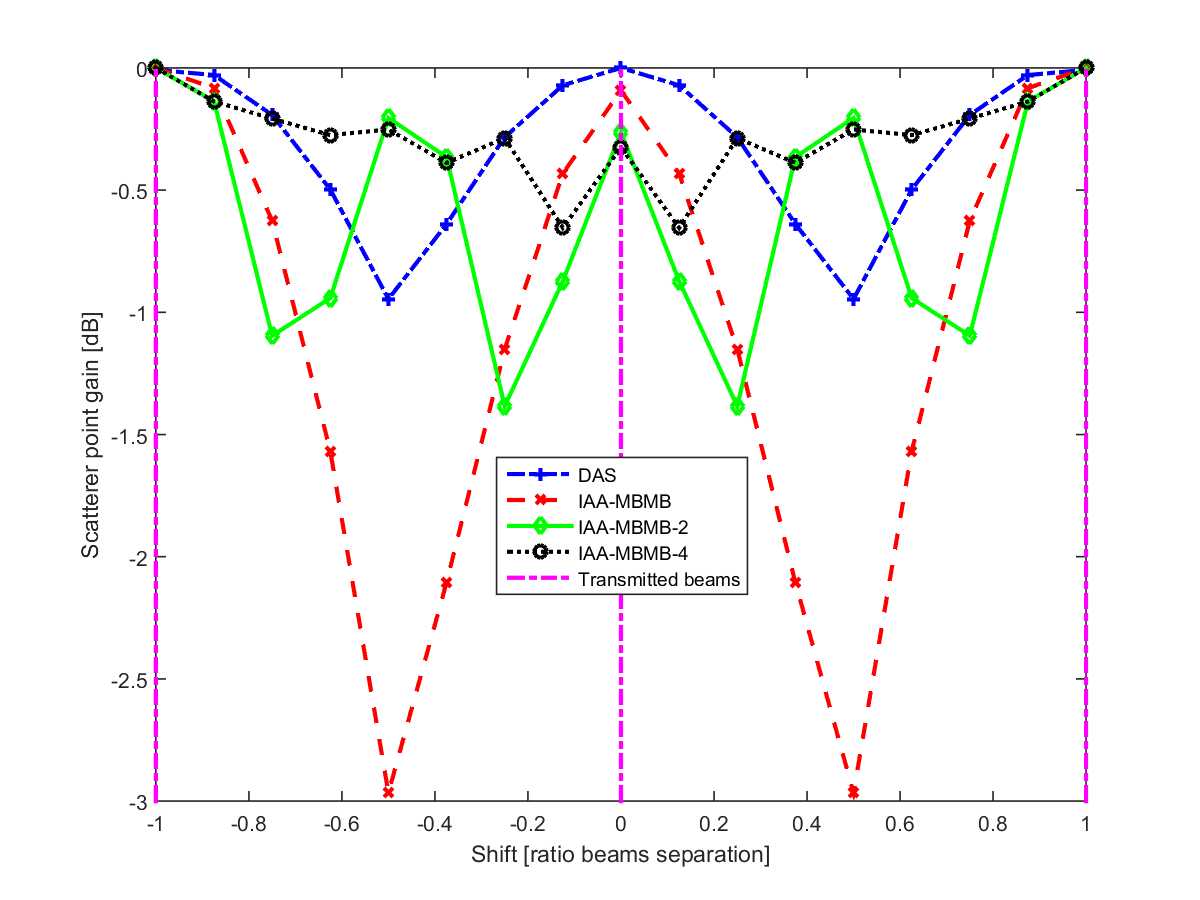
\includegraphics[width=\linewidth]{./images/discussion/loss_vs_shift_upsampled.png}
    \end{subfigure}
    \quad
    \begin{subfigure}[t]{0.48\linewidth}
        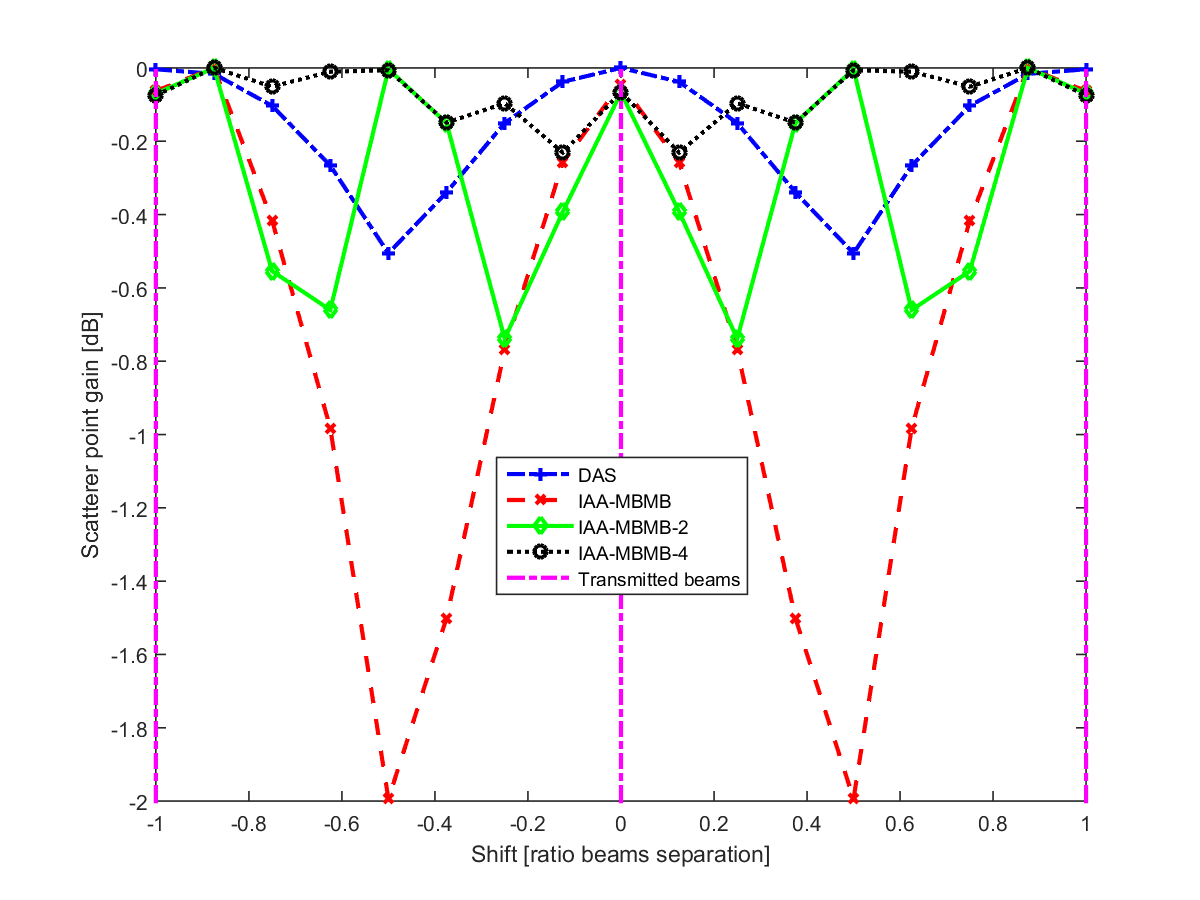
\includegraphics[width=\linewidth]{./images/discussion/loss_vs_shift_50mm_upsampled.png}
    \end{subfigure}
	\caption{Maximum gain of single point moving at respectively 40 (left) and 50 (right) mm radius}
	\label{fig:loss_vs_shift_upsampled}
\end{figure}

\begin{figure}[ht]
    \centering
    \begin{subfigure}[t]{0.48\linewidth}
        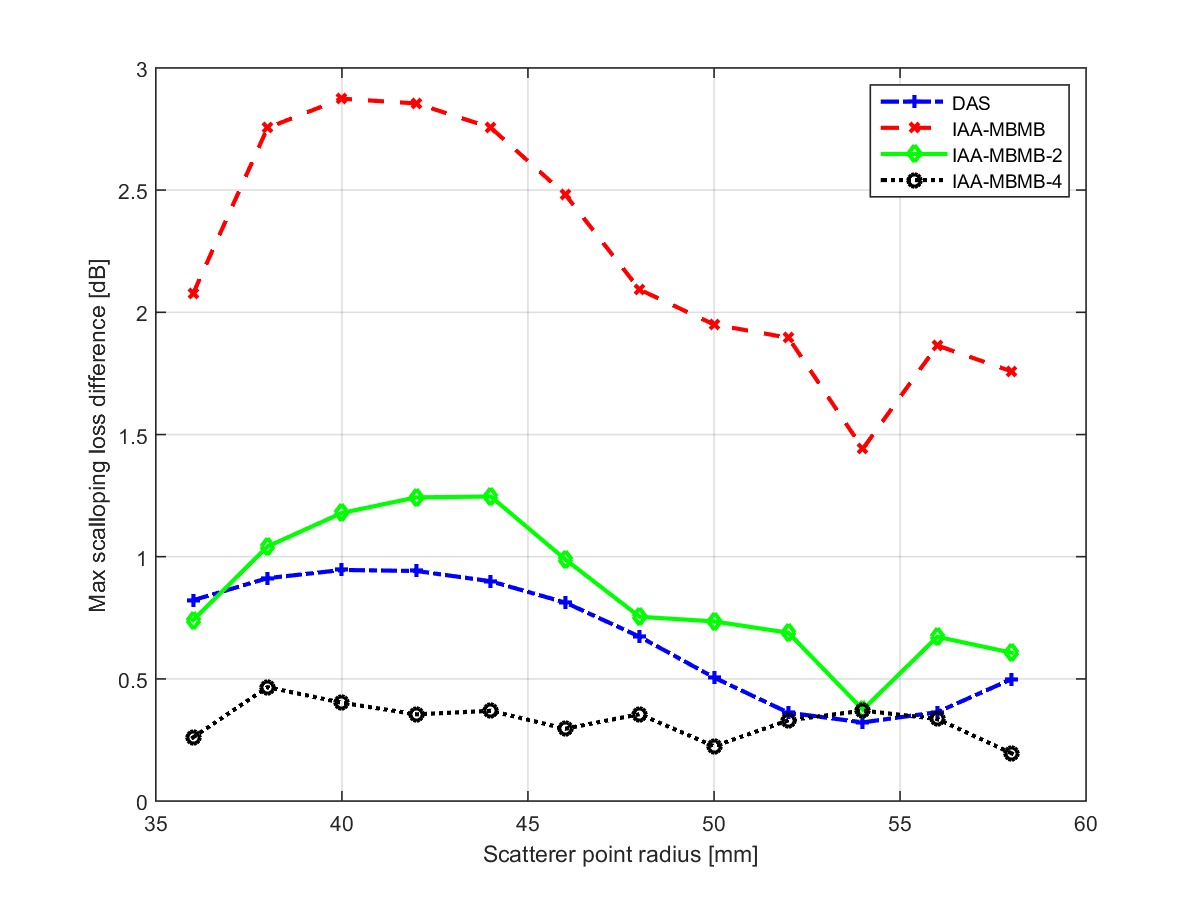
\includegraphics[width=\linewidth]{./images/discussion/loss_vs_range_upsampled.png}
    \end{subfigure}
    \quad
    \begin{subfigure}[t]{0.48\linewidth}
        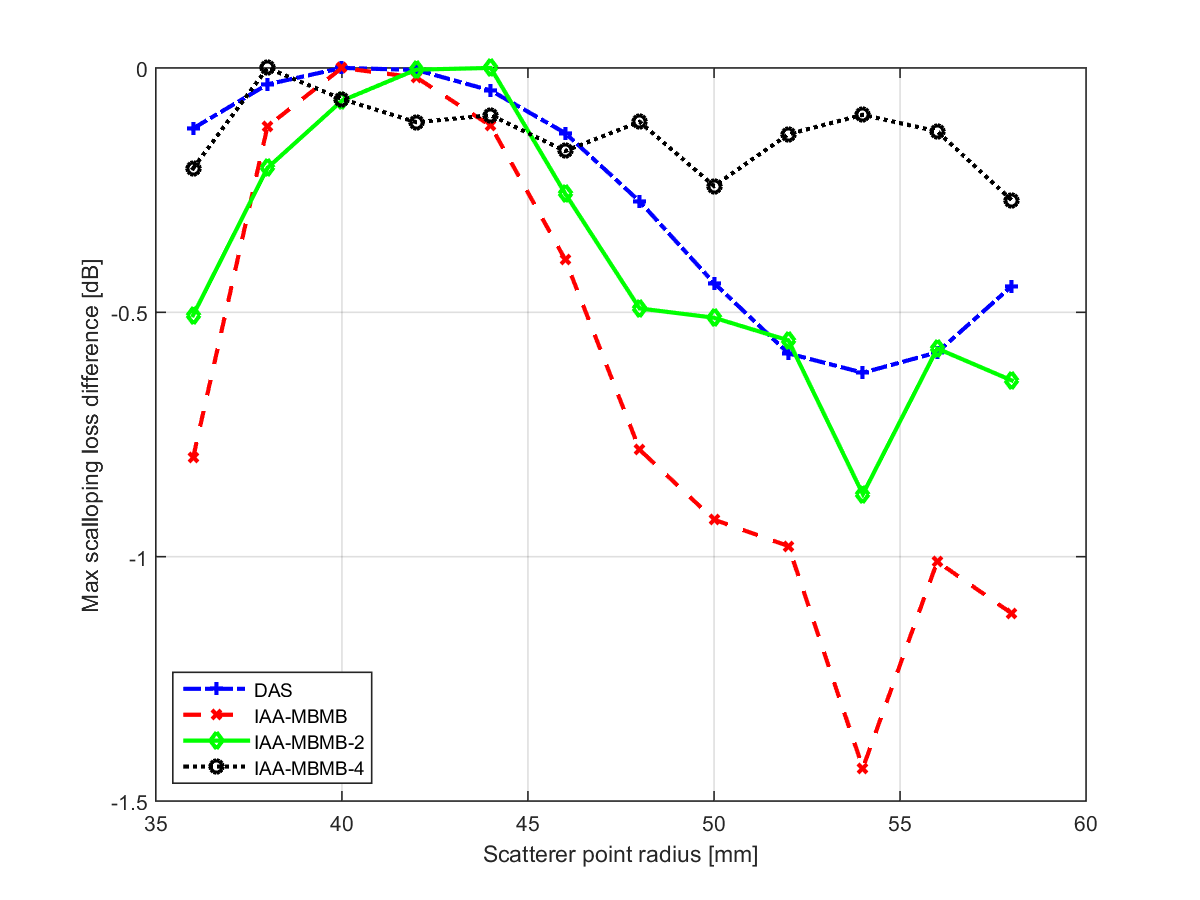
\includegraphics[width=\linewidth]{./images/discussion/loss_vs_range_upsampled_diff.png}
    \end{subfigure}
	\caption{Maximum scalloping loss of single point moving at constant radius. The right figure displays the normalized curves}
	\label{fig:loss_vs_range_upsampled}
\end{figure}

\begin{figure}[ht]
    \centering
    \begin{subfigure}[t]{0.48\linewidth}
        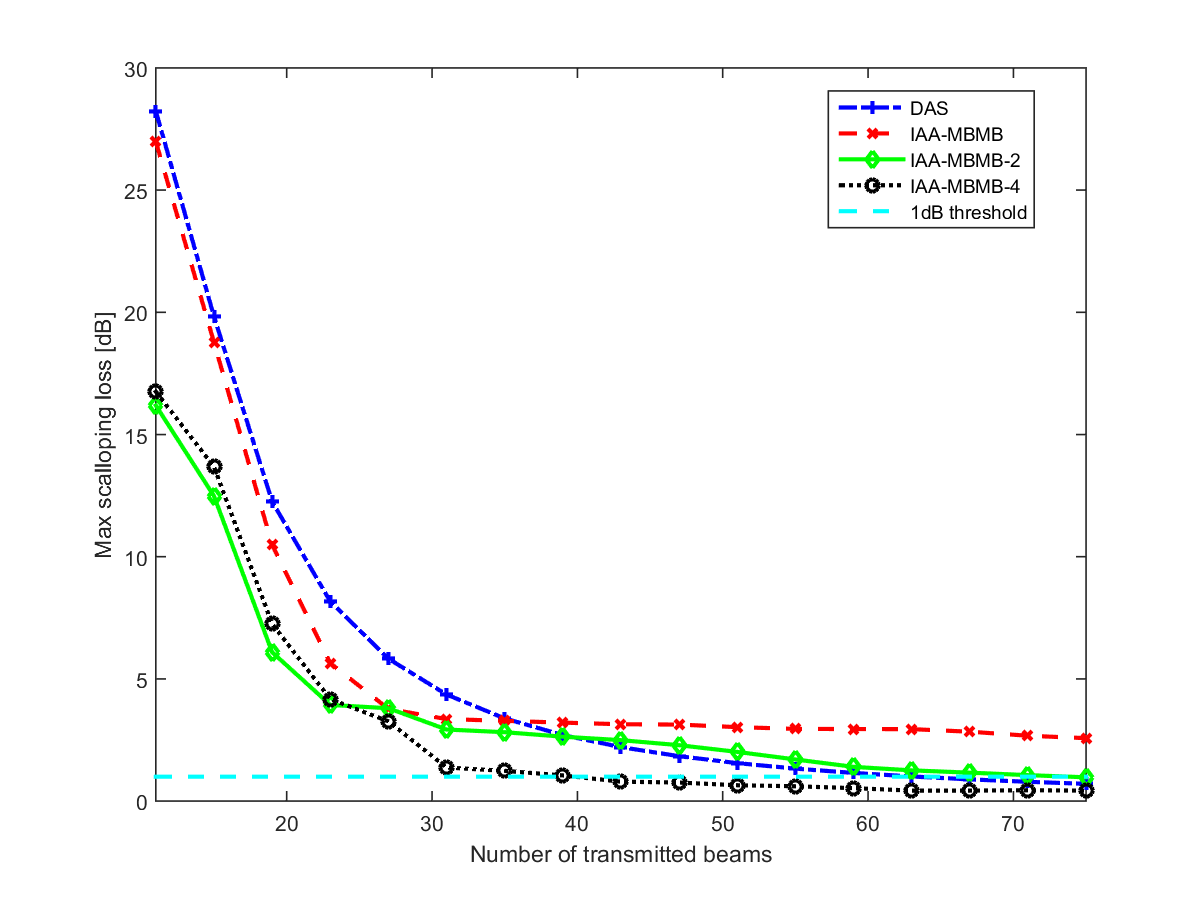
\includegraphics[width=\linewidth]{./images/discussion/loss_vs_beams_upsample.png}
    \end{subfigure}
    \quad
    \begin{subfigure}[t]{0.48\linewidth}
        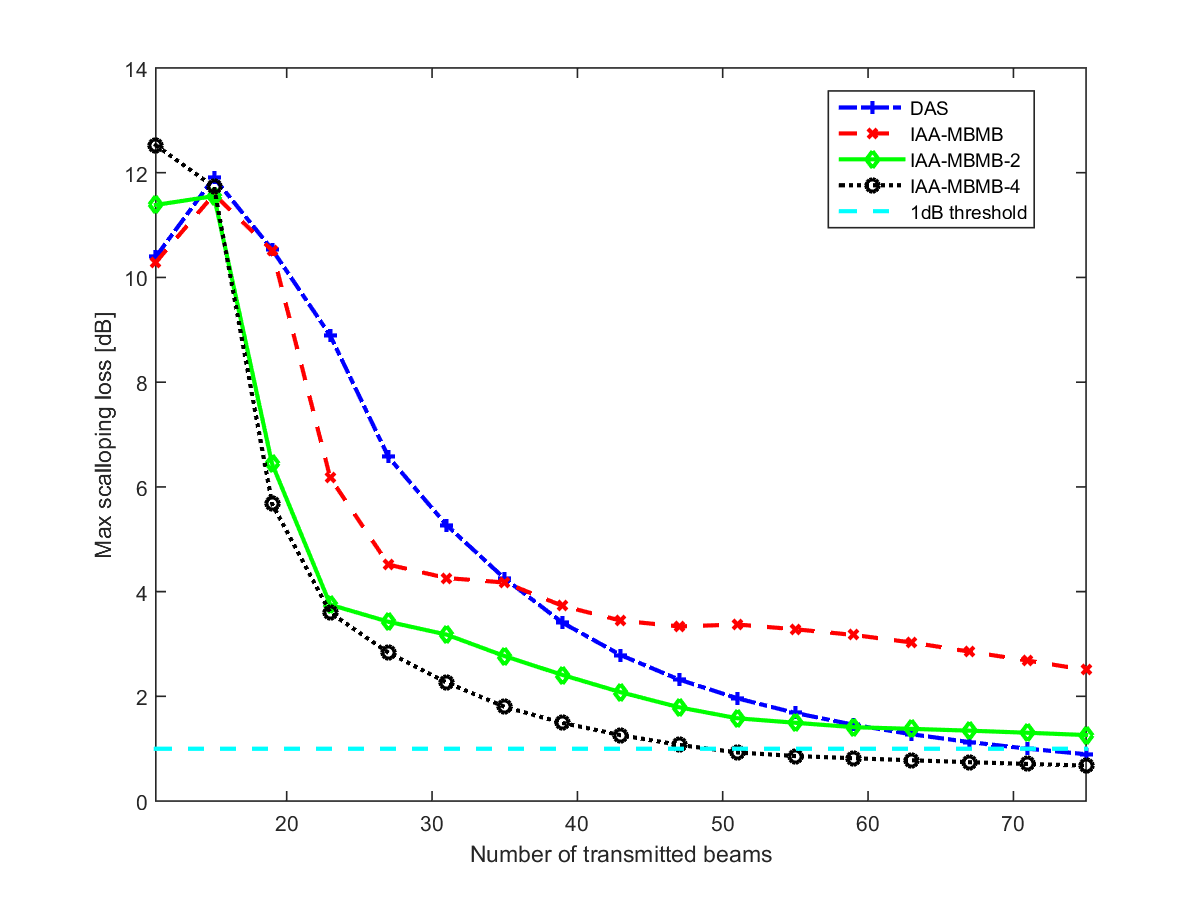
\includegraphics[width=\linewidth]{./images/discussion/loss_vs_beams_speckle_upsample.png}
    \end{subfigure}
	\caption{Maximum scalloping loss versus number of transmit beams a) in a noise-less medium, b) in speckle noise}
	\label{fig:loss_vs_beams_upsample}
\end{figure}

With this new approach to estimating the maximum scalloping loss, Figure \ref{fig:loss_vs_beams_upsample} displays the estimated maximum scalloping loss for various transmit beam densities, both in a noise-less medium and with presence of speckle noise. 
Figure \ref{fig:loss_vs_beams_upsample} reveals that, as expected, phased-based upsampling reduces the effects of scalloping loss. The IAA-MBMB-2 and IAA-MBMB-4 methods require even fewer transmit beams than the DAS beamformer. The difference in number of transmit beams requirements between the two scenario also seems to scale down as $F_{up}$ increases. This could mean that the use of phase-based upsampling is able to reduce the influence of the medium properties on the scalloping loss magnitude.
Tables \ref{table:num_beams_upsample} and \ref{table:frame_rate_upsample} are summing up the information from Figure \ref{fig:loss_vs_beams_upsample} in the same manner as in Section \ref{sec:res_frames_motion}.

\begin{table}[!ht]
\centering
\begin{tabular}{| c | c | c | c |}
  \hline
  Beamformer &   Without speckle   &   Speckle - seed 2 &   Speckle - seed 42 \\
  \hline
  DAS           &   65      &   75  &    \\
  IAA-MBMB      &   141     &   91  &    \\
  IAA-MBMB-2    &   75     &    111 &    \\
  IAA-MBMB-4    &   41     &    51  &    \\
  \hline
 \end{tabular}
\caption{Required number of transmit beams for non-visible scalloping loss}
\label{table:num_beams_upsample}
\end{table}

\begin{table}[!ht]
\centering
\begin{tabular}{| c | c | c | c |}
  \hline
  Beamformer &   Without speckle   &    Speckle - seed 2 &   Speckle - seed 42 \\
  \hline
  DAS           &   76.92      &   66.66  &    \\
  IAA-MBMB      &   34.48     &   49.5  &    \\
  IAA-MBMB-2    &   66.66     &         &    \\
  IAA-MBMB-4    &   121.95     &  98.04 &    \\
  \hline
 \end{tabular}
\caption{Maximum frame rate to guarantee no visible scalloping loss}
\label{table:frame_rate_upsample}
\end{table}

The phase-based upsampling approach has proven to be a very useful tool for increasing a beamformer frame rate. 
A similar analysis than Section \ref{sec:res_beams_motion} remains to be done for this approach in order to discover any potential artifacts resulting from its use. Figures \ref{} reiterate the experiments done in Section \ref{sec:res_beams_motion}.

\begin{figure}[ht]
    \centering
    \begin{subfigure}[t]{0.48\linewidth}
        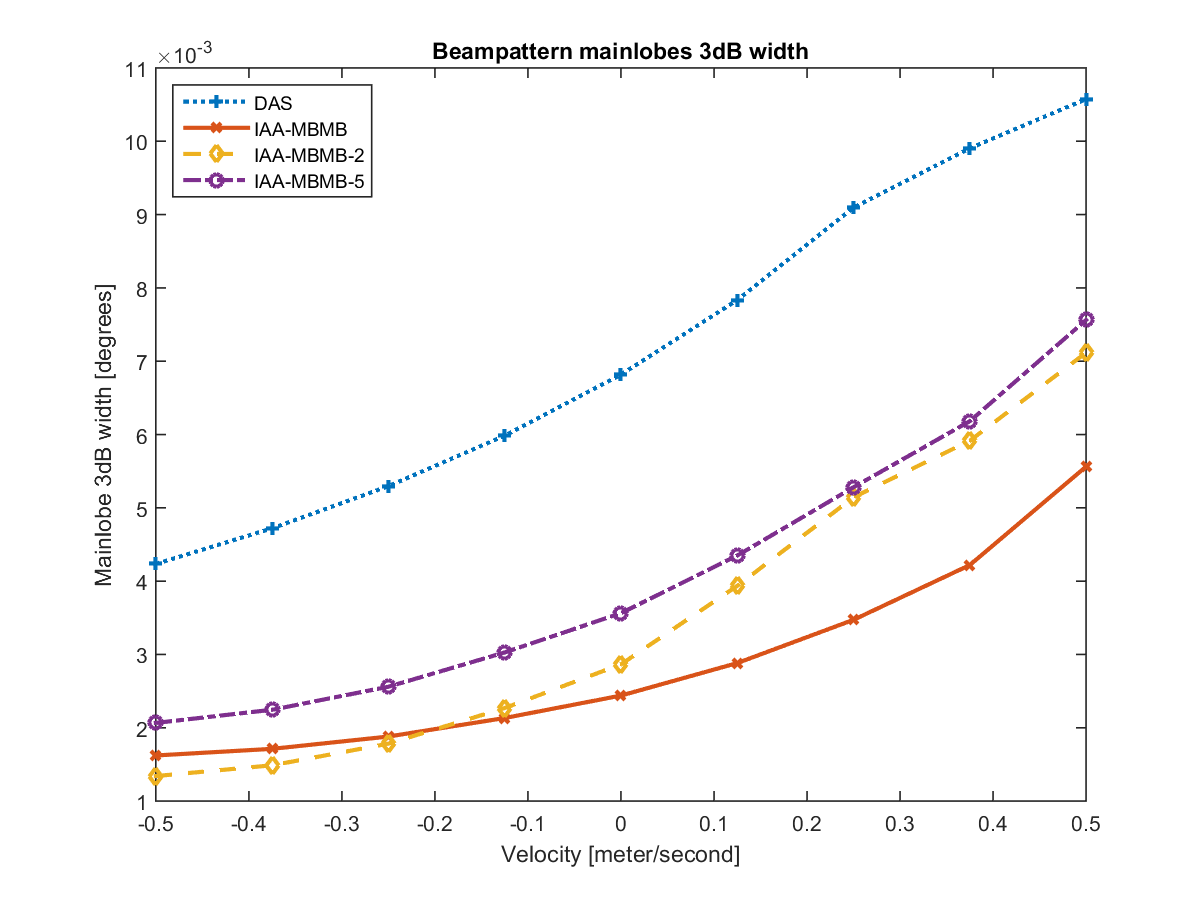
\includegraphics[width=\linewidth]{./images/discussion/mainlobe_vs_speed.png}
    \end{subfigure}
    \quad
    \begin{subfigure}[t]{0.48\linewidth}
        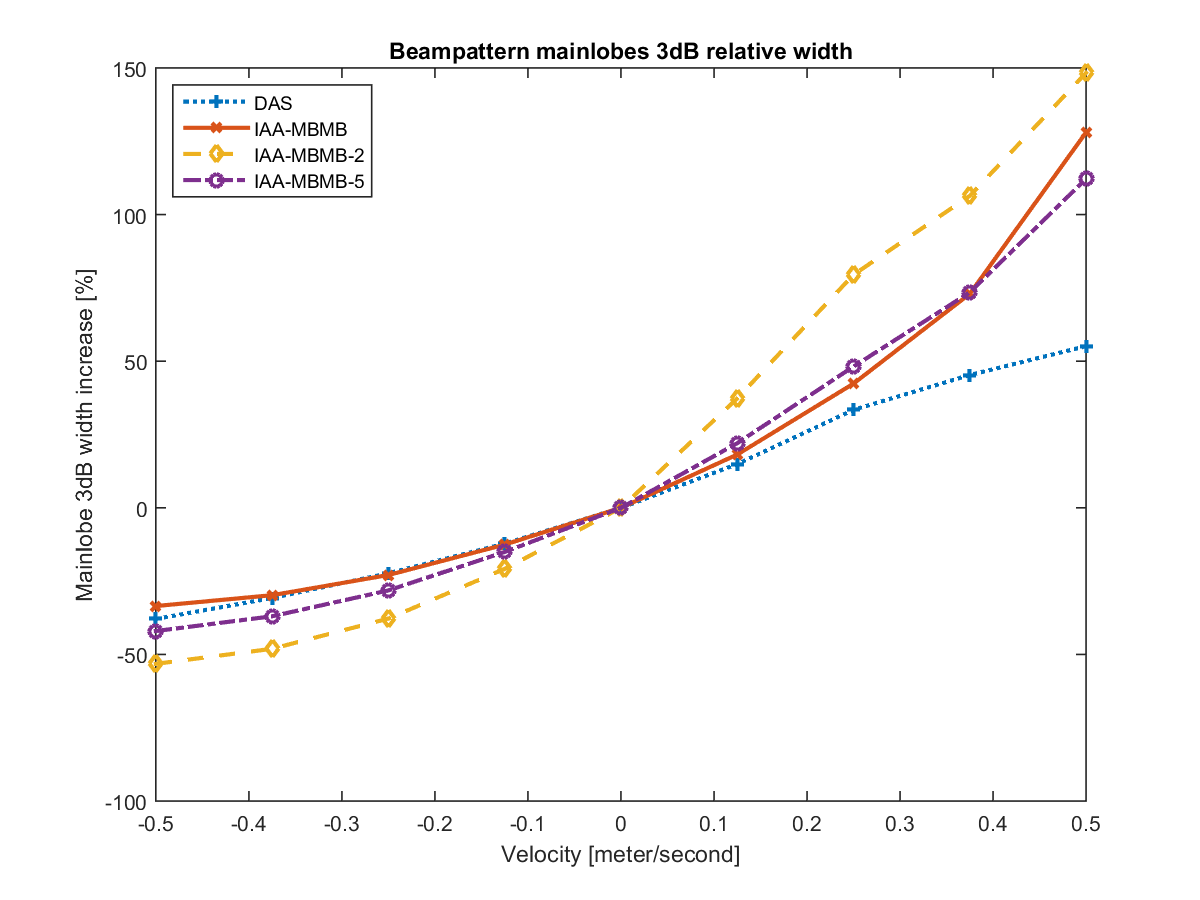
\includegraphics[width=\linewidth]{./images/discussion/mainlobe_vs_speed_relative.png}
    \end{subfigure}
	\caption{Steering  response  mainlobe  width  versus  scatterer  point velocity. The right plot shows their relative increase}
	\label{fig:mainlobe_vs_speed_upsample}
\end{figure}

\begin{figure}[ht]
    \centering
    \begin{subfigure}[t]{0.48\linewidth}
        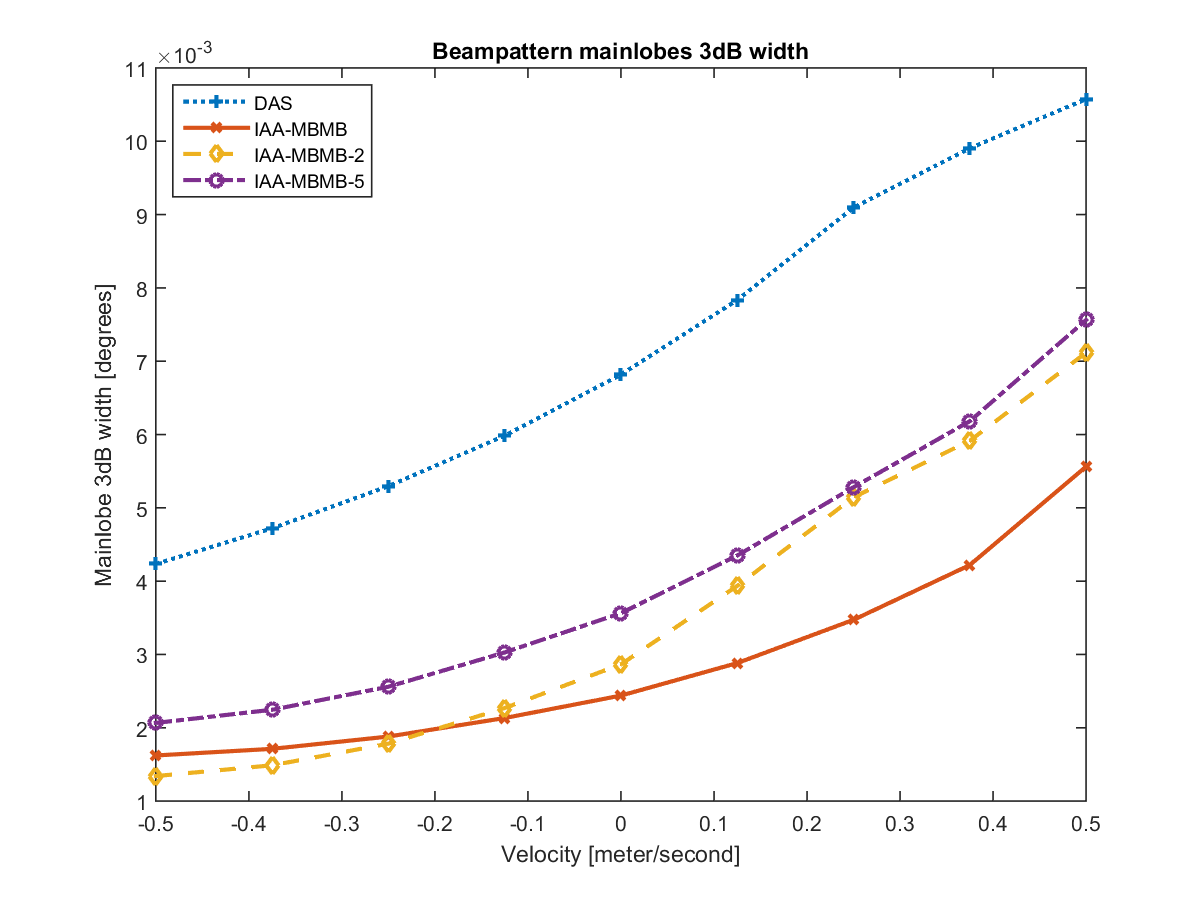
\includegraphics[width=\linewidth]{./images/discussion/mainlobe_vs_speed.png}
    \end{subfigure}
    \quad
    \begin{subfigure}[t]{0.48\linewidth}
        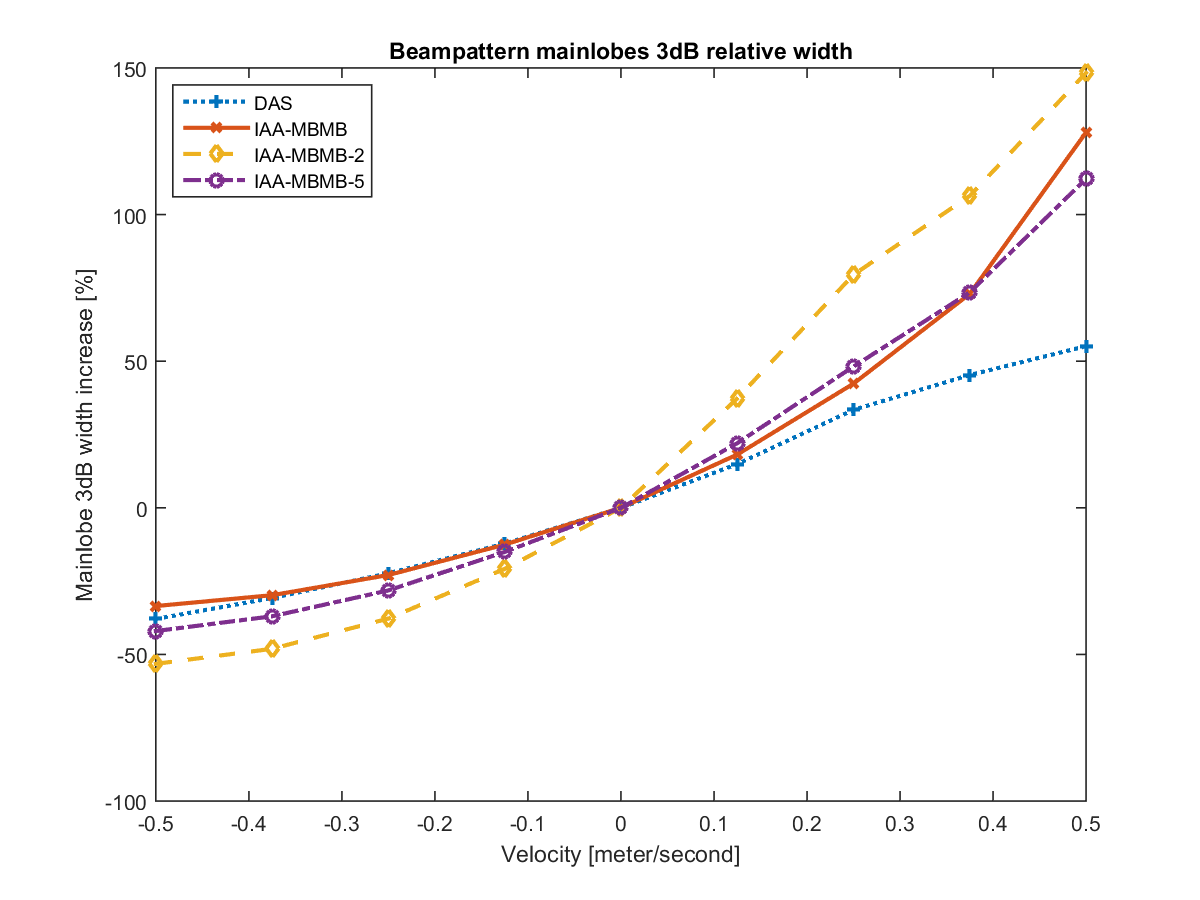
\includegraphics[width=\linewidth]{./images/discussion/mainlobe_vs_speed_relative.png}
    \end{subfigure}
    \quad
    \begin{subfigure}[t]{0.48\linewidth}
        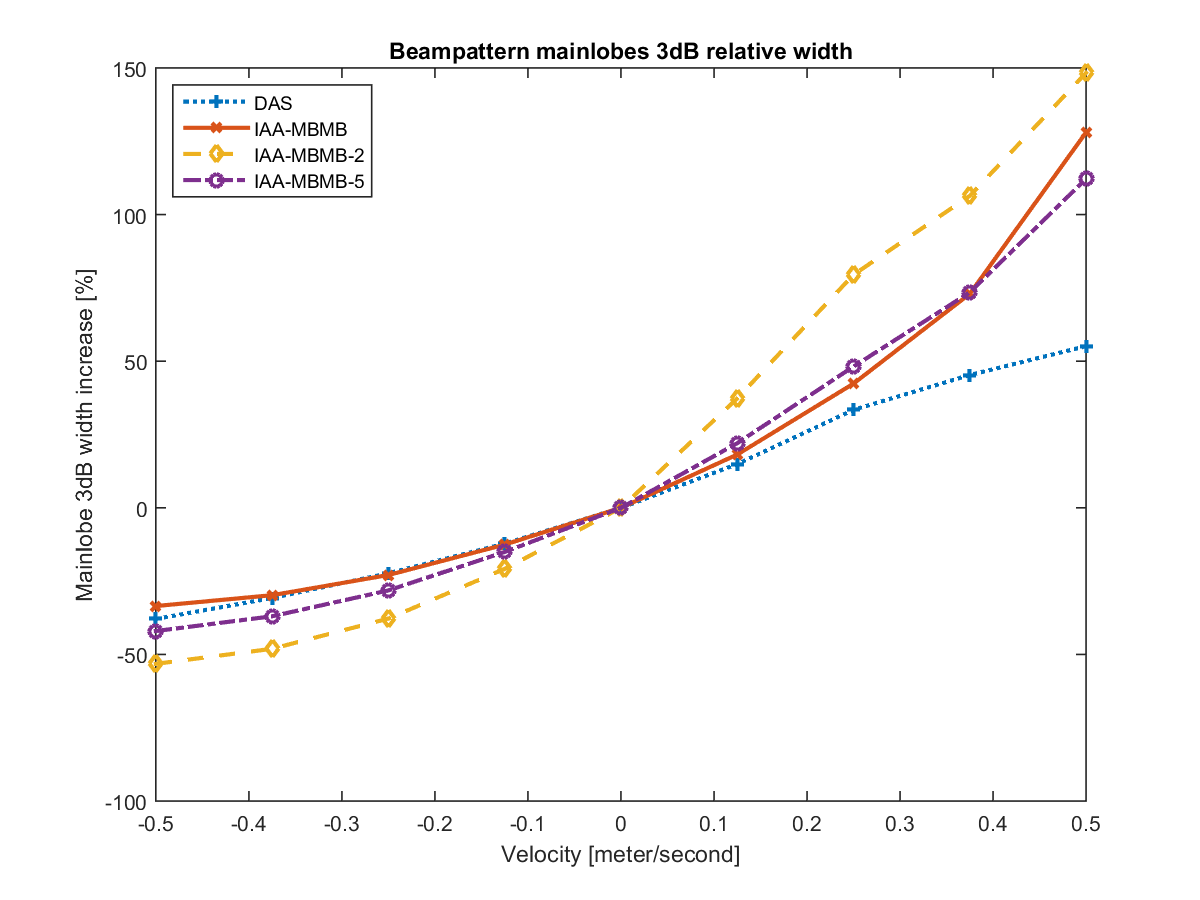
\includegraphics[width=\linewidth]{./images/discussion/mainlobe_vs_speed_relative.png}
    \end{subfigure}
    \quad
    \begin{subfigure}[t]{0.48\linewidth}
        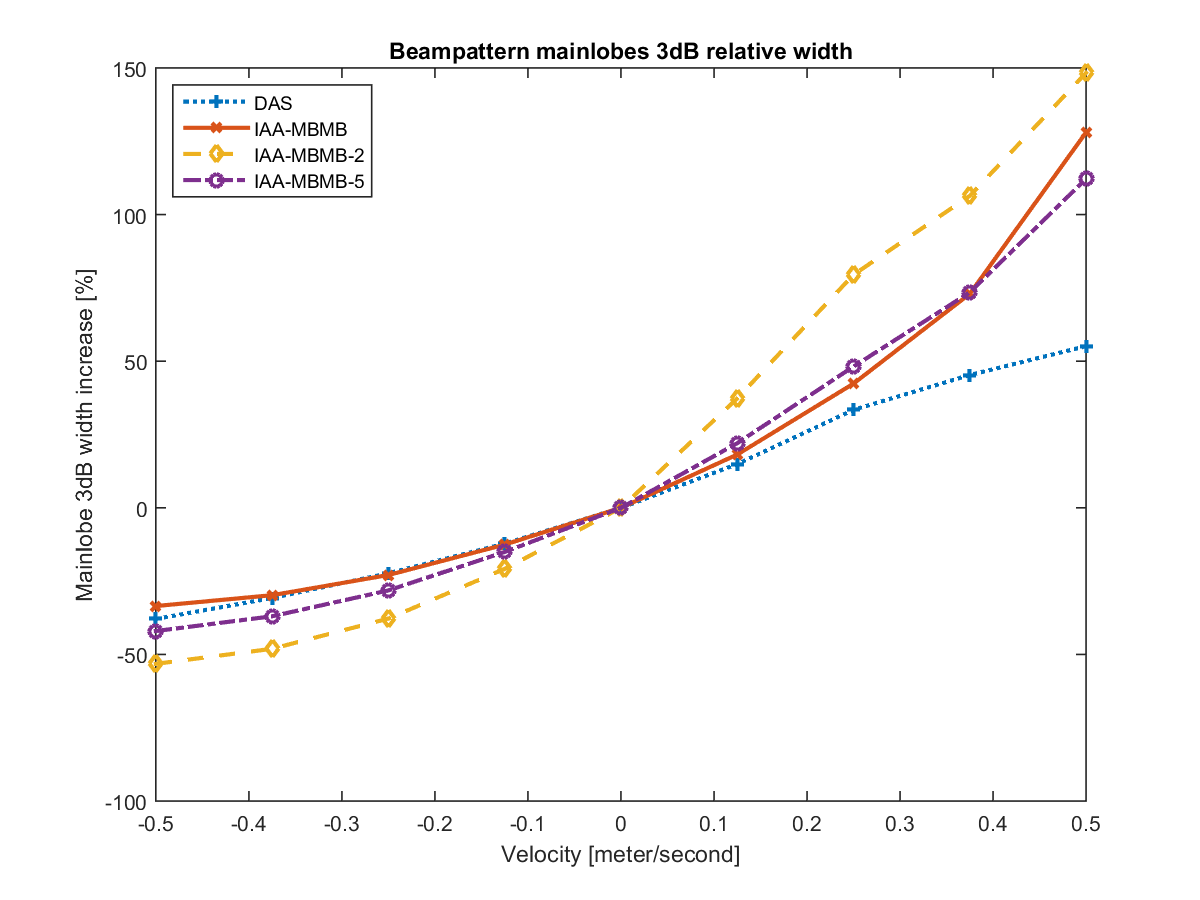
\includegraphics[width=\linewidth]{./images/discussion/mainlobe_vs_speed_relative.png}
    \end{subfigure}
	\caption{Steering  response  mainlobe  width  versus  scatterer  point velocity. The right plot shows their relative increase}
	\label{fig:mainlobe_vs_speed_upsample}
\end{figure}
\fi
